\documentclass[final,5p,times,twocolumn]{elsarticle}
\usepackage[T1]{fontenc}
\usepackage{microtype,graphicx,booktabs,amsmath,amssymb,amsthm,array,tabularx,multirow}
\usepackage{xcolor,tikz,pgfplots,enumitem,placeins,xurl}
\usetikzlibrary{arrows.meta,positioning,calc,fit,matrix,backgrounds}
\pgfplotsset{compat=1.18}
\usepackage[hypertexnames=false]{hyperref}
\urlstyle{same}
\hypersetup{hidelinks,pdfauthor={Chengzhan Li},pdftitle={Phase-Scoped Query Layouts for Reference-Preserving Speculative Decoding}}
\definecolor{target}{HTML}{426B8B}
\definecolor{draft}{HTML}{B07B43}
\definecolor{qualified}{HTML}{3E725E}
\definecolor{aux}{HTML}{6B7075}
\definecolor{light}{HTML}{EDF1F3}
\newcommand{\QB}{\mathrm{QB}}
\newcommand{\PQ}{\mathrm{PQ}}
\newcommand{\GS}{\mathrm{GS}}
\newcommand{\MQ}{\mathrm{MQ}}
\newtheorem{proposition}{Proposition}
\newcolumntype{Y}{>{\raggedright\arraybackslash}X}
\setlength{\emergencystretch}{2em}
\renewcommand{\bibfont}{\small}
\raggedbottom
\setlength{\tabcolsep}{4pt}
\renewcommand{\arraystretch}{1.12}
\setlist{nosep,leftmargin=*}
\tikzset{box/.style={draw=aux,rounded corners=2pt,align=center,inner sep=5pt,font=\small},flow/.style={-{Latex[length=2mm]},line width=.6pt,draw=aux}}

\begin{document}
\begin{frontmatter}
\title{Phase-Scoped Query Layouts for Reference-Preserving Speculative Decoding}
\author{Chengzhan Li}
\address{University of Electronic Science and Technology of China, Chengdu, China\\[2pt]
{\normalfont\ttfamily\href{mailto:chengzhan.li@std.uestc.edu.cn}{chengzhan.li@std.uestc.edu.cn}}}
\begin{abstract}Speculative verification changes query batching and can alter the greedy output of a quantized deployment. We present a phase-scoped query-to-batch (QB) transformation that preserves query and mask indexing, shares K/V storage and makes the layout part of graph reuse while retaining batched projections and feed-forward computation. A six-session CUDA experiment spanning two dates reduces speculative request latency relative to explicit per-query attention (PQ) by 3.06\%, 6.17\% and 2.83\% for Qwen3, SmolLM2 and Llama, with complete reference-output agreement on the fixed panel. A separate 72-context replay finds bitwise PQ/QB correspondence at QK, softmax and AV. Vulkan state interventions expose component-substitution limits; a scoped backend port subsequently preserves the reference on real grouped-query verification requests. Controlled mapping experiments show that CUDA Graph replay and representation costs can remove apparent optimization opportunities, while a cheaper padded path can fail the specified reference. Two new four-input, fresh-context service panels qualify real two-query verification but establish no practical QB-over-PQ benefit: the point reductions are 1.07\% on RTX and 0.49\% on B570, with the RTX estimate unresolved under 5.21\% identical-control imbalance. Speculative service is 41.8\% lower than target-only service in the RTX panel and 2.62 times as costly in the B570 panel under their respective frozen policies. These results separate a reference-preserving representation, its implementation cost and the net value of drafting, and identify the state and backend conditions required for transfer.
\end{abstract}
\begin{keyword}
speculative decoding \sep execution geometry \sep numerical consistency \sep runtime graph transformation \sep state composition
\end{keyword}
\end{frontmatter}
\section{Introduction}
Speculative decoding saves sequential target invocations by verifying several draft tokens together~\cite{leviathan2023,chen2023}. That change also alters the target's execution geometry. Floating-point evaluation can depend on query width, so mathematically equivalent batching can change the greedy response of a deployed quantized model. When an application must retain its existing regression baseline, recovering the reference output becomes part of the optimization problem.

The decisive choice is where to impose that numerical constraint. Global serialization (GS) evaluates one target row at a time through projections, attention and feed-forward layers. It recovers a serial execution organization at the cost of surrounding batching. Per-query attention (PQ) confines the separation to attention but constructs a subgraph for each query. We ask whether the same local organization can be expressed more cheaply, and whether the resulting repair changes the economic case for drafting.

Phase-scoped query-to-batch attention (QB) answers the first question through graph lowering. It views Q as $(d,1,h,q)$ instead of $(d,q,h,1)$ and transforms the mask in parallel. Existing attention operators process the queries as separate batch instances while K/V storage remains shared within one sequence. Projections and feed-forward computation stay batched. Role/phase guards and a layout-sensitive graph cache bind this representation to the native speculative transaction, including execution with observation disabled.

The contribution is this runtime contract and its measured consequences. Query independence itself is standard attention structure. Batch-invariant kernels control reductions~\cite{thinkingmachines}; CoRun controls prefill and decode shapes~\cite{corun}; LLM-42 verifies a fast path under a fixed-shape schedule~\cite{llm42}. QB instead preserves a local one-query attention organization through views, head mapping, phase dispatch and graph reuse, without adding a numerical-consistency verifier. Section~\ref{sec:related} compares these control points explicitly.

The matched CUDA experiments separate three decisions. First, local repair changes drafting from a net cost to a net benefit for Qwen3 and Llama; both PQ and QB cross this boundary. Second, QB lowers the representation cost within local repair: six sessions across two dates yield speculative PQ/QB request-time ratios of 1.032, 1.066 and 1.029 for Qwen3, SmolLM2 and Llama. A 72-context replay finds bitwise agreement at QK, softmax and AV. Third, a cheaper representation does not guarantee profitable drafting: SmolLM2 benefits from QB but remains faster without the draft.

Transfer and deployment test the same argument at larger boundaries. Vulkan state interventions show that endpoint-equivalent states can contain noninterchangeable KV components. A grouped-query port preserves the existing AV evaluation while dispatching independent queries. Finally, mapping and fresh-context service studies measure the complete transaction~\cite{mappingrecords,b570servicerecords,rtxservicerecords}. Neither fresh-context panel establishes a practical QB/PQ increment. Their different net draft costs reinforce the need to compare qualified policies at the intended request boundary.

The contributions are:
\begin{enumerate}[label=(\arabic*),itemsep=2pt]
\item A phase-scoped attention transformation with paired Q/mask views, shared-KV and head semantics, ordered output recovery and layout-sensitive graph reuse.
\item Matched evidence that repair scope changes draft profitability, followed by a separate measurement of QB's incremental cost benefit over PQ.
\item State and backend transfer tests, together with measurements of the representation benefit at the deployment request boundary.
\end{enumerate}
The supplement supplies the full comparisons, failures and implementation records; ancillary files pin their source identities~\cite{studyrecords}.

\section{Reference contract and execution model}
\label{sec:contract}
\subsection{Output qualification}
Let $\rho$ identify the reference model and tokenizer bytes, prompt construction, numerical runtime, ordinary execution recipe, sampler and stopping rule. For input $x$, its endpoint is
\begin{equation}
\mathcal O_\rho(x)=(\mathbf y,\mathbf e,n,y_{\mathrm{last}},s),
\label{eq:endpoint}
\end{equation}
where $\mathbf y$ is the full native token-ID array, $\mathbf e$ its end-of-generation (EOG) flags, $n$ its length and $s$ the stop reason. The principal campaigns stop at native EOG or 128 generated tokens. A candidate qualifies on a registered panel $X$ when every required pair has $\mathcal O_c(x)=\mathcal O_\rho(x)$, the reference is stable and all required records are present. A shorter divergent response cannot qualify a latency comparison.

We distinguish exact-arithmetic equivalence, bitwise operator correspondence and endpoint agreement. Each answers a different question. Backend acceptance and actual operator placement are additional execution prerequisites. These definitions apply throughout the paper; qualification always refers to the stated configuration, panel and output window.

\subsection{The stateful transaction}
A target context owns KV values, sequence positions, a pending sampled token or available logits, and relevant sampler state. The draft has separate state. It proposes up to $k$ tokens; the target evaluates the pending token and proposal positions; acceptance, correction and any bonus determine the committed prefix. Rejected positions are reconciled before the next cycle. A visible token may still be pending evaluation into KV and must be consumed exactly once.

QB changes the target attention representation inside this transaction. It adds no numerical-consistency verifier; the ordinary speculative verification and reconciliation still execute. Microbatch capacity $U$, occupied query count $q$, caller width and output reservation remain distinct. We write UB$n$ for a configured capacity of $n$. A caller containing $k+1$ rows can execute as several physical micrographs, so caller counts alone do not describe parallel work.

\subsection{Local repair and state composition}
The design objective is to minimize complete request time over tested implementations, subject to endpoint qualification. Write a request fragment as $D_g(P_g(x))$, where $P_g$ forms the state consumed by $D_g$ under execution organization $g$. Correspondence of $D_{\QB}$ and the reference on one input state $s_\rho$ does not establish correspondence on the different state $P_g(x)$.

For full stateful composition, a relation between candidate and reference states must hold initially, preserve the committed output at each transaction, and hold again after reconciliation. This is a standard sufficient-condition argument; its premises are tested empirically here. Section~\ref{sec:state} examines two simpler assumptions often used in local reasoning: that endpoint-equivalent states have interchangeable components, and that enlarging a sufficient replacement preserves its effect.

\section{Phase-scoped query-layout design}
\label{sec:method}
\subsection{Separating attention from target-wide batching}
Figure~\ref{fig:design} contrasts the three repair organizations. GS processes target rows one at a time throughout projection, attention and the feed-forward network. PQ retains batched surrounding work but explicitly constructs an attention subgraph for each query and concatenates the results. QB retains that local one-column organization through a view: queries become separate batch instances of the existing attention operators. It does not serialize the surrounding layers or construct a distinct attention subgraph per query.

\begin{figure*}[t]
\centering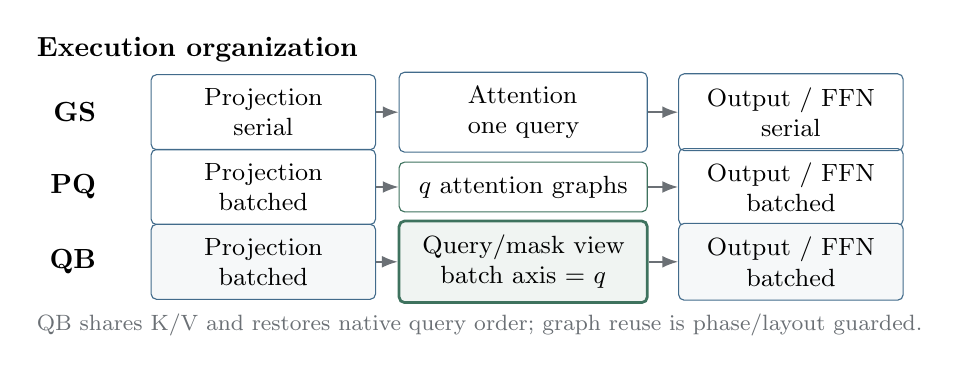
\begin{tikzpicture}[x=1cm,y=1cm,font=\small]
\node[anchor=west,font=\bfseries] at (0,3.3) {Execution organization};
\foreach \y/\lab in {2.5/GS,1.55/PQ,.6/QB} {
  \node[anchor=east,font=\bfseries] at (1.0,\y) {\lab};
}
\node[box,draw=target,text width=2.5cm] (g1) at (3,2.5) {Projection\\serial};
\node[box,draw=target,text width=2.8cm] (g2) at (6.3,2.5) {Attention\\one query};
\node[box,draw=target,text width=2.5cm] (g3) at (9.7,2.5) {Output / FFN\\serial};
\node[box,draw=target,text width=2.5cm] (p1) at (3,1.55) {Projection\\batched};
\node[box,draw=qualified,text width=2.8cm] (p2) at (6.3,1.55) {$q$ attention graphs};
\node[box,draw=target,text width=2.5cm] (p3) at (9.7,1.55) {Output / FFN\\batched};
\node[box,draw=target,fill=target!5,text width=2.5cm] (b1) at (3,.6) {Projection\\batched};
\node[box,draw=qualified,fill=qualified!8,text width=2.8cm,line width=1pt] (b2) at (6.3,.6) {Query/mask view\\batch axis = $q$};
\node[box,draw=target,fill=target!5,text width=2.5cm] (b3) at (9.7,.6) {Output / FFN\\batched};
\foreach \a/\b in {g1/g2,g2/g3,p1/p2,p2/p3,b1/b2,b2/b3}\draw[flow] (\a)--(\b);
\node[anchor=west,text=aux,font=\footnotesize] at (0,-.2) {QB shares K/V and restores native query order; graph reuse is phase/layout guarded.};
\end{tikzpicture}

\caption{Three same-reference implementation alternatives. Boxes show logical graph organization, not measured kernel occupancy. QB changes attention representation while keeping surrounding target computation batched. Numbered query and mask tiles depict logical indexing, not copied K/V or independent sequences. Phase selection is part of graph construction and reuse; the speculative transaction is unchanged.}
\label{fig:design}
\end{figure*}

We label the ordinary graph with multiple query positions MQ; this denotes execution geometry, not the multi-query attention (MQA) architecture with one shared K/V head. The intervention point follows the native Q/K/V permutations in the non-flash attention builder. Let $d$ be the query/key channel dimension, $q$ the number of occupied queries, $h_Q$ the query-head count, and $n$ the key extent. Using the runtime's axis order, the input query has shape $(d,q,h_Q, 1)$. QB creates a four-dimensional view with shape $(d, 1,h_Q,q)$ and preserves the original query-column stride as the new fourth-axis stride. This is a view of the same input values, not a different projection or a re-encoding of the tokens.

\subsection{Address, mask and head semantics}
Write the original byte strides as $s_0,s_1,s_2,s_3$ and the base pointer as $b_Q$. For channel $i$, head $a$ and logical query $j$, the original address is
\begin{equation}
\operatorname{addr}_{\MQ}(i,j,a, 0)=b_Q+i s_0+j s_1+a s_2.
\end{equation}
The transformed view satisfies
\begin{equation}
\operatorname{addr}_{\QB}(i, 0,a,j)=b_Q+i s_0+a s_2+j s_1,
\label{eq:address}
\end{equation}
so it selects the same scalar. The singleton query-column stride is immaterial for access, but the implementation still supplies a valid native view descriptor. It must not invent a contiguous layout when the source is strided.

The mask is transformed in parallel from $(n,q, 1,1)$ to $(n, 1,1,q)$. For original mask strides $m_0,m_1$, query $j$ still reads $b_M+t m_0+j m_1$ for key index $t$. The original mask values, including padded or disallowed positions, are retained. Changing the view must not replace a query-dependent causal mask by a single shared column. Logical token positions are unchanged: the new batch coordinate labels queries in one sequence, not independently positioned sequences.

Let $\kappa(a)$ denote the native grouped-query head mapping from query head $a$ to a K/V head. Under an integral grouped-query ratio, the same mapping is used by all three organizations. K and V retain their native values, strides and single-stream ownership and broadcast over the new query-batch coordinate. In mathematical notation, for the already implemented scaling $\alpha$ and admissible mask $m$,
\begin{align}
 z_{tja}&=\alpha\sum_i K_{it\kappa(a)}Q_{ija}+m_{tj},\\
 p_{tja}&=\frac{\exp(z_{tja})}{\sum_u\exp(z_{uja})},\\
 O_{vja}&=\sum_t V_{vt\kappa(a)}p_{tja}.
\label{eq:attn}
\end{align}
These equations describe logical indices; the actual runtime may store or permute V differently. QB must retain that implementation's mapping rather than reinterpret V by this notation alone.

\begin{proposition}[Mathematical view equivalence]
For a supported single-stream attention graph, suppose Equation~\eqref{eq:address} and the corresponding mask mapping hold, K/V broadcasting preserves $\kappa$, operator parameters are unchanged, and output recombination restores query order. In exact arithmetic, QB and the original attention graph compute the same logical $O$ in Equation~\eqref{eq:attn}.
\end{proposition}
\begin{proof}
For each fixed $(j,a)$, both representations select identical Q, K, V and mask values. The sums range over the same channel and key indices, and softmax is normalized over the same keys. The batch label in QB separates query instances but changes neither their operands nor their logical dependence. Recombination restores $(v,j,a)$ order. Thus every logical output value agrees in exact arithmetic. Finite-precision correspondence is established separately by the operator and complete-output experiments.
\end{proof}

After QK, softmax and AV, the native contiguous recombination restores the target's expected query/head order before its batched output projection. PQ realizes the same mathematical separation by slicing one query and its mask column per subgraph. The question tested later is whether QB matches PQ's \emph{observed numerical execution} without paying for the same subgraph structure.

\subsection{Admission conditions are part of the method}
The evaluated build admits one sequence/KV stream, non-flash attention, supported Qwen3 or dense Llama-family graph paths, compatible head dimensions, an integral GQA ratio, F32 query/mask values and F16 K/V. At most four queries are occupied in the current QB study. Attention bias, sinks and MLA value projections are excluded by the relevant source guards; other positional-bias schemes or unsupported strides require separate handling and validation. The mask may contain padded columns, but its first $q$ logical query columns and original key extent must be represented correctly.

These conditions preserve distinct meanings for sequence ownership, query indexing and head grouping. Additional streams need their own batch coordinate; biases and sinks need their own broadcasting rules. The source guards enforce the supported feature set, and each backend validates operator admission. Wider-geometry and fused-attention paths have separate numerical and execution contracts (\sref{supp:implementation}).

\subsection{Phase binding and graph-cache consistency}
The transformation is selected by a process-fixed four-bit mask: target prefill, target continuation, draft prefill and draft continuation have bits 1, 2, 4 and 8. Mask 3 enables the two target phases. A scoped guard derives the active flag from the current role and phase, places that flag in graph parameters, and restores its prior value on exit. New requests reset the phase to prefill. Crucially, this guard executes before the observation-disabled fast path returns to native decoding; turning off a diagnostic callback must not disable the repair.

Graph caching creates a second obligation. Two calls can share nominal capacity and tensor extents yet require different attention layouts. The active-layout flag therefore participates in the reuse check. A mismatch rejects reuse and requires an appropriate graph. The original campaigns fix the implementation choice (QB, PQ or GS) within each process. The later matched native bridge uses separate contexts for each layout within a process (Section~\ref{sec:matchedbridge}). Both keep the implementation fixed within a context; they do not validate dynamic PQ/QB switching under one cached graph. Table~\ref{alg:scope} summarizes the dispatch and reuse checks.

\begin{table}[t]
\caption{Phase-scoped dispatch and reuse obligations.}
\label{alg:scope}
\begin{tabularx}{\columnwidth}{@{}rX@{}}\toprule
1 & On request reset, establish target/draft ownership and set phase to prefill.\\
2 & Compute the role/phase bit and save the previous scope flag.\\
3 & Set the active flag before both observed and unobserved decode paths.\\
4 & If cached topology's layout flag differs, reject reuse.\\
5 & For an active supported attention graph, apply Q/mask views, native QK--softmax--AV and ordered recombination.\\
6 & Otherwise retain the declared untransformed graph or reject an unsupported active case.\\
7 & Complete native acceptance/state updates and restore the prior scope flag.\\\bottomrule
\end{tabularx}
\end{table}

The surrounding operators remain batched. Complete-output qualification therefore tests the transformation within its numerical stack, including state formed upstream. The Vulkan projection interventions in Section~\ref{sec:state} locate this producer-side dependency.

\subsection{Selecting the active phases}
A prior four-switch experiment tested all 16 masks on four exposed HumanEval inputs at $k=3$, UB4 and cap128. Masks 3, 7, 11 and 15 passed both repetitions; mask3 was inclusion-minimal within that finite mask family. It was then fixed for the later model-family tests. The complete pattern and the separate mask3/mask15 cost comparison appear in \sref{supp:implementation}; that comparison did not pass its practical speed threshold.

\section{Experimental design}
\label{sec:experiments}
\subsection{Systems, panels and distinct evidence roles}
The implementation uses pinned llama.cpp/GGML sources~\cite{llamacpp,studyrecords}. CUDA experiments run on an RTX~5070~Ti Laptop GPU with Q8\_0 target/draft pairs: Qwen3-8B/0.6B~\cite{qwen3}, SmolLM2-1.7B-Instruct/135M-Instruct, and Llama-3.1-8B-Instruct/3.2-1B-Instruct. The models share a backend but include different head dimensions and attention-head mappings. Weight files and runtime libraries are byte-pinned, with exact versions recorded in the ancillary source manifest.

The ordinary CUDA reference uses physical UB1. Repaired execution uses target caller UB4, draft UB1, $k=3$, F16 KV, non-flash attention and context size 1024. The requested logical batch of 2048 is clamped to 1024; the frontend uses 24 host threads. One request is active at a time and prompt-cache reuse is disabled. The original Vulkan state studies instead use an Arc~B570 and Llama-3.1-8B-Instruct Q6\_K, with F16 KV, context 1024 and ten host threads. They are state and portability experiments, not a controlled comparison of GPU speed.

The core CUDA panels use sanitized MBPP and GSM8K inputs~\cite{mbpp,gsm8k}; HumanEval supplies engineering and Vulkan service probes~\cite{humaneval}. The new-input transfer panel adds CodeContests programming tasks~\cite{rtxtransferrecords}. Outcomes are response preservation and runtime. Table~\ref{tab:campaigns} maps each panel to its research question and distinguishes repeated execution from new-input validation.

\begin{table*}[t]\centering\small
\caption{Principal evidence groups. Counts include the indicated repeats, not independent tasks. Exact sources, failure records and access scope are indexed in \sref{supp:reproduction}.}
\label{tab:campaigns}
\begin{tabularx}{\textwidth}{@{}>{\raggedright\arraybackslash}p{2.6cm}>{\raggedright\arraybackslash}p{5.2cm}Y@{}}\toprule
Study & Design & Question answered\\\midrule
CUDA output confirmation & 24 project-unused inputs per family; 5 arms; 2 sessions; 5 repeats; 3,600 requests & Complete-output qualification of a frozen repair and ordinary baselines\\
CUDA repair comparison & 12 exposed inputs per family; 7 arms; 2 sessions; 4 repeats; 2,016 formal requests & PQ/QB/GS costs and matched draft increment\\
CUDA E2 replication & Same 12-input panel; 6 separated sessions; 324 fresh workers; 1,620 requests including 324 warmups & Independent-process PQ/QB comparison across two dates; retrospective local draft-on/off analysis\\
CUDA E1 replay & 3 families $\times$ 3 layers $\times$ 2 phases $\times$ 4 query widths; 216 model requests and 432 replays & Same-input QK, softmax and AV correspondence\\
Vulkan state studies & Prefill partitioning, admitted whole-state crosses, and 32 controls plus 160 subset requests & State formation and component substitution\\
Vulkan port and source audit & Stopped natural pilot; 432 synthetic CPU fixtures and frozen support-predicate analysis & Endpoint counterexamples and backend admission\\
Later mapping studies & RTX replay/padding controls and independent B570 representation transactions & Mapping admissibility under a strong software baseline\\
Fresh-context service panels & Four exposed inputs and four process sessions per platform; separate references and policies & Real two-query execution, layout cost and draft economics\\
Matched CUDA deployment & 12 exposed Qwen3 inputs; $k=1,3$ by resident/fresh; 6 process sessions on one date; 864 measurements and 72 warmups & Layout benefit under matched draft length and request lifecycle\\
New-input CUDA transfer & 12 inputs planned per family; 33/36 family/input cells reached; 4 sessions per qualified family; 384 measurements and 384 warmups & Qwen3/SmolLM2 qualification and cost on all 12 inputs each; Llama stops at a reference counterexample\\\bottomrule
\end{tabularx}
\end{table*}

The 24-input output-confirmation panel was frozen after exclusion against accessible project execution history. The repair comparison and E2 reuse 12 exposed texts, six from each domain; the matched deployment study retains the Qwen3 panel. E1 selects one exposed prompt per family before capture. The new-input transfer panel is frozen separately after exclusion against project history. Vulkan state interventions use two known divergent inputs, two stable controls and separately labelled synthetic prefixes. Each panel supports the claim listed in Table~\ref{tab:campaigns}.

\subsection{Matched alternatives and complete-request timing}
The seven repair-comparison arms are $R$, $M_{\QB}$, $C_{\QB}$, $M_{\PQ}$, $C_{\PQ}$, $M_{\GS}$ and $C_{\GS}$. $M$ is target-only; $C$ adds the same draft protocol. GS physically serializes active target rows without changing the registered draft or stopping rule. PQ and QB retain surrounding batching. The original campaign uses arm-specific workers and reverses their order in its second session. E2 retains $R$ and the four PQ/QB arms, using two serial-reference endpoints for each task/session.

The paid CUDA interval is a complete nonstreaming resident-process HTTP request, including encoding/submission, generation, response parsing and endpoint validation. Model loading, artifact writes, hashes and registered warmups are outside it. The counts channel adds no heavy tensor readback or observation synchronization. Diagnostic times are separate and are not subtracted from request measurements.

For task $i$, session $s$ and arms $a,b$, let $t_{i,s,a}$ be the registered request measurement, or the within-session median where repetitions are specified. We use equal task and session log weights:
\begin{equation}
S_{a/b}=\exp\!\left(\frac{1}{|\mathcal S|}\sum_s\frac{1}{|X|}\sum_i\log\frac{t_{i,s,a}}{t_{i,s,b}}\right).
\label{eq:ratio}
\end{equation}
Values above one favor the denominator. Full required pairs must qualify; missing and divergent records are retained without imputation. On a common paired panel, ratio products obey algebraic identities, but they do not decompose operator time.

E2 uses fresh processes, short PQ/QB blocks and counterbalanced order. Six sessions span 24.45 hours from first to last start, with at least one hour between a completion and the next start. The primary interval is the registered pointwise 95\% percentile bootstrap of six session-level log contrasts, using 10,000 resamples. Its sampling unit is the session and its target is the fixed 12-input panel on one host. The practical ratio threshold is 1.02: for PQ/QB, this corresponds to a QB latency reduction of $1-1/1.02\approx1.96\%$. The later service studies register a 2\% reduction relative to their PQ control mean. No request-level bootstrap, outlier trimming or significance-dependent stopping is used.

A secondary sensitivity analysis applies a two-sided Student $t_5$ interval to the same six session mean log contrasts and recomputes the estimate after omitting each session. The $t$ interval assumes independent, approximately normal session log means. It checks dependence on the interval method and individual sessions while retaining the registered bootstrap as primary.

The retrospective E2 draft-on/off analysis pairs the four local arms within each family/task/session. It applies the same equal log weights to $M_L/C_L$ and reports exploratory pointwise $t_5$ intervals across six session means. These contrasts were not preregistered, and their intervals provide no simultaneous-coverage guarantee. They use no additional requests and leave the registered PQ/QB estimands and intervals unchanged.

\subsection{Numerical and state controls}
E1 freezes actual Q/K/V/mask bytes, shapes, strides, head maps and parameters. Native MQ capture/replay correspondence, within-arm repeatability and capture-on/off endpoint equality precede PQ/QB comparison. Each of 72 fresh workers runs a counts warmup, a heavy capture and a counts observer control; MQ, PQ and QB are then replayed twice per context. A failed control withholds the corresponding numerical claim.

Vulkan interventions reconstruct a declared continuation boundary: complete sequence KV and positions, initial full FP32 logits consumed by the native greedy sampler, an empty generated prefix and correct pending-token ownership. Sixteen own-path shams precede whole-KV crosses. Subset tests retain recipient initial logits and verify actual imported bytes. Subsequent four-cell analyses compare full logits only at a shared consumed prefix.

The service and mapping studies specify their own reference and cost windows (Sections~\ref{sec:service} and \ref{sec:mappingcosts}); the matched deployment design changes $k$ and lifecycle within a common runtime (Section~\ref{sec:matchedbridge}). Campaign identities, amendments and execution dispositions are indexed in the supplement. The resident HTTP comparisons retain their stated $k=3$ policy, timer and task weights.

\section{Repair scope and query-layout cost}
\label{sec:results}
\subsection{Repair scope changes draft profitability}
\label{sec:economics}
The seven-arm campaign compares repair scope and drafting on the same 12-input panel. All seven arms qualify 96/96 complete endpoints per family under the declared reference. Figure~\ref{fig:cost} separates local representation cost, global serialization cost and the draft increment under all three repair organizations. These estimates retain the original two-session protocol, separately from E2.

\begin{figure*}[t]\centering
\resizebox{\textwidth}{!}{\begin{tikzpicture}
\begin{groupplot}[group style={group size=3 by 1,horizontal sep=.70cm},
width=.305\textwidth,height=5.6cm,ymin=.5,ymax=3.5,ytick={1,2,3},
tick label style={font=\footnotesize},title style={font=\small,yshift=12pt},label style={font=\footnotesize,align=center},
axis lines*=left,axis line style={aux,line width=.45pt},tick style={aux},grid=major,grid style={gray!13}]
\nextgroupplot[title={\textbf{A} Local representation},xlabel={$T_{C_{\PQ}}/T_{C_{\QB}}$\\$>1$: QB faster},xmin=.995,xmax=1.09,xtick={1,1.04,1.08},yticklabels={Llama,SmolLM2,Qwen3}]
\addplot[aux,dashed] coordinates {(1,.5)(1,3.5)};
\addplot[only marks,mark=diamond*,mark size=2.7pt,qualified] coordinates {(1.043676000000,3)};
\node[font=\scriptsize,anchor=south] at (axis cs:1.043676000000,3.12){1.044};
\addplot[only marks,mark=diamond*,mark size=2.7pt,qualified] coordinates {(1.068111000000,2)};
\node[font=\scriptsize,anchor=south] at (axis cs:1.068111000000,2.12){1.068};
\addplot[only marks,mark=diamond*,mark size=2.7pt,qualified] coordinates {(1.021848000000,1)};
\node[font=\scriptsize,anchor=south] at (axis cs:1.021848000000,1.12){1.022};
\nextgroupplot[title={\textbf{B} Global serialization},xlabel={$T_{C_{\GS}}/T_{C_{\QB}}$\\$>1$: QB faster},xmin=.95,xmax=2.55,xtick={1,1.5,2,2.5},yticklabels={,,}]
\addplot[aux,dashed] coordinates {(1,.5)(1,3.5)};
\addplot[only marks,mark=diamond*,mark size=2.7pt,qualified] coordinates {(2.143525000000,3)};
\node[font=\scriptsize,anchor=south] at (axis cs:2.143525000000,3.12){2.144};
\addplot[only marks,mark=diamond*,mark size=2.7pt,qualified] coordinates {(1.462530000000,2)};
\node[font=\scriptsize,anchor=south] at (axis cs:1.462530000000,2.12){1.463};
\addplot[only marks,mark=diamond*,mark size=2.7pt,qualified] coordinates {(2.175941000000,1)};
\node[font=\scriptsize,anchor=south] at (axis cs:2.175941000000,1.12){2.176};
\nextgroupplot[title={\textbf{C} Draft value by repair},xlabel={$D_L=T_{M_L}/T_{C_L}$\\$>1$: drafting faster},xmin=.53,xmax=1.27,xtick={.6,.8,1,1.2},yticklabels={,,},legend style={at={(.5,1.01)},anchor=south,draw=none,font=\scriptsize,fill=none},legend columns=3]
\addplot[aux,dashed,forget plot] coordinates {(1,.5)(1,3.5)};
\addplot[only marks,mark=square*,mark size=2.4pt,aux] coordinates {(0.709722260013,3.23) (0.592109590630,2.23) (0.724338602453,1.23)};
\addlegendentry{GS}
\addplot[only marks,mark=o,mark size=2.4pt,target] coordinates {(1.125118952936,3.00) (0.616360145288,2.00) (1.107396133613,1.00)};
\addlegendentry{PQ}
\addplot[only marks,mark=diamond*,mark size=2.4pt,qualified] coordinates {(1.143749000000,2.77) (0.633948000000,1.77) (1.116620000000,0.77)};
\addlegendentry{QB}
\end{groupplot}
\end{tikzpicture}
}
\caption{Matched repair and drafting choices in the original seven-arm campaign, separate from E2. A/B: speculative PQ and GS costs relative to QB. C: draft value under each repair organization, $D_L=T_{M_L}/T_{C_L}$; values above one favor drafting. Qwen3 and Llama cross parity under both local repairs, while SmolLM2 remains below it. GS/PQ values in C are reconstructed by Equation~\ref{eq:draft} from the common-panel ratios. All points are descriptive estimates; exact source ratios and every regression are retained in \sref{supp:cost}.}
\label{fig:cost}
\end{figure*}

Its speculative GS/QB ratios are 2.144, 1.463 and 2.176; every task favors QB. These differences reflect the value of constraining attention locally while retaining batched projection and feed-forward work. The PQ/QB ratios, 1.044, 1.068 and 1.022, measure the representation choice within local repair. These common-panel estimates distinguish repair scope from layout cost; E2 supplies a separately scheduled PQ/QB comparison.

A retrospective audit of all 2,016 formal responses forms 288 matched seven-arm audit groups. All 1,728 within-path GS/PQ/QB pairings agree in recorded proposals, acceptance, logical rows, rollback and caller-width histograms; complete native token IDs and recorded EOG flags match the paired $R$ endpoints. GS changes physical batching as intended; PQ/QB agree in every workload field. This holds recorded logical work fixed without apportioning operator time (\sref{supp:sevenarmwork}).

Adding the draft to QB is profitable for Qwen3 and Llama but not SmolLM2: $M_{\QB}/C_{\QB}$ is 1.144, 0.634 and 1.117. SmolLM2 takes about 1.58 times its own draft-free request duration despite QB being cheaper than PQ. Across the common seven-arm panel, draft value under another layout $L$ follows
\begin{equation}
D_L=\frac{S_{M_L/M_{\QB}}}{S_{C_L/C_{\QB}}}\,D_{\QB},\qquad D_{\QB}=S_{M_{\QB}/C_{\QB}}.
\label{eq:draft}
\end{equation}
The derived GS/PQ/QB values are 0.710/1.125/1.144 for Qwen3, 0.592/0.616/0.634 for SmolLM2 and 0.724/1.107/1.117 for Llama. Thus the repair policy changes the sign of the observed draft decision for two families. Both PQ and QB cross the profitability boundary; their direct comparison measures QB's additional layout benefit.

The relative change in draft value summarizes this interaction:
\begin{equation}
\Gamma_{\QB\leftarrow\GS}=\frac{D_{\QB}}{D_{\GS}}
=\frac{S_{C_{\GS}/C_{\QB}}}{S_{M_{\GS}/M_{\QB}}}.
\label{eq:repairinteraction}
\end{equation}
It is 1.612, 1.071 and 1.542 for the three families, respectively. These are retrospective ratio-of-ratios summaries from the reported common-panel estimates, with the original weights and timer. They quantify how repair policy changes the draft increment at complete-request level. The draft's incremental cost must therefore be evaluated under the repair policy being considered.

Reference-preserving batching also has value without drafting. Target-only QB lowers cost relative to the specified serial reference: $R/M_{\QB}$ is 1.334051, 1.369890 and 1.426161, with every task favoring QB on this panel. For SmolLM2, the measured choice is therefore to retain target-only QB batching and omit the draft. These complete-request gains include prompt prefill; the target-only continuation uses a common one-query path. They establish neither a single-token decoding speedup nor a measured decomposition by phase.

A historical fixed-UB4 experiment provides a related counterexample: increasing $k$ from 3 to 7 preserved outputs but reduced request speed to 0.890 of the smaller-draft path. Separate work captures recorded fewer target callers and more physical micrographs. Acceptance and caller reduction alone therefore cannot establish request acceleration. The width failures and negative cost results that constrain this conclusion remain in \sref{supp:implementation}.

\subsection{Draft decisions across the six E2 sessions}
\label{sec:e2draft}
E2 records target-only and speculative requests under each local layout. We retrospectively pair its 864 non-warmup local-arm measurements into 216 family/task/session quartets: $M_{\PQ}$, $M_{\QB}$, $C_{\PQ}$ and $C_{\QB}$. The contrast $D_L=S_{M_L/C_L}$ uses the weights in Equation~\ref{eq:ratio}.

\begin{table}[t]\centering\small
\caption{Retrospective E2 draft values on the fixed 12-input panel: $D_L=T_{M_L}/T_{C_L}>1$ favors drafting. QB intervals are exploratory pointwise 95\% $t_5$ intervals over six session log means. E2 has no GS arm.}\label{tab:e2draft}
\begin{tabular}{@{}lrrr@{}}\toprule
Family & $D_{\mathrm{PQ}}$ & $D_{\mathrm{QB}}$ & QB interval\\\midrule
Qwen3 & 1.072 & 1.084 & [1.059, 1.109]\\
SmolLM2 & 0.576 & 0.597 & [0.582, 0.612]\\
Llama & 1.091 & 1.105 & [1.097, 1.113]\\
\bottomrule\end{tabular}
\end{table}


Table~\ref{tab:e2draft} retains all three local-policy directions: drafting benefits Qwen3 and Llama, while SmolLM2 favors target-only execution. Every one of the six session estimates has the corresponding direction under both PQ and QB. Under QB, drafting reduces complete-request latency by 7.72\% and 9.51\% for Qwen3 and Llama; it increases SmolLM2 latency by 67.52\%. The magnitudes differ from the original two-session campaign, while the policy decisions agree.

The exploratory pointwise $t_5$ intervals use sessions as sampling units; the registered PQ/QB analysis is unchanged. Pairing separately collected target-only and speculative blocks does not remove within-session drift. Without a GS arm, E2 checks the local draft decision rather than independently replicating the full repair-scope interaction. Complete estimates and the PQ-to-QB change in draft value appear in \sref{supp:e2draft}.

\subsection{QB's independent implementation benefit}
\label{sec:e2}
The registered E2 comparison isolates representation cost within local repair. It completes 1,620 requests in 324 fresh workers, including 324 warmups and 432 serial-reference measurements. There are no request failures, output mismatches, workload errors or heavy-observer flags. The six-session speculative ratios $C_{\PQ}/C_{\QB}$ are 1.031614, 1.065803 and 1.029114, corresponding to 3.06\%, 6.17\% and 2.83\% lower QB request latency. Figure~\ref{fig:e2} shows both paths and their session-level uncertainty.

Table~\ref{tab:e2absolute} gives absolute costs from the source-verified requests, using the same task/session log weights.
\begin{table}[t]\centering\small
\caption{Absolute E2 request costs (ms), with equal task and session weights in the geometric mean. Registered warmups are excluded; the paid interval includes submission, full-response parsing and endpoint validation.}\label{tab:e2absolute}
\begin{tabular}{lrrrr}
\toprule
Family & $M_{\mathrm{PQ}}$ & $M_{\mathrm{QB}}$ & $C_{\mathrm{PQ}}$ & $C_{\mathrm{QB}}$ \\
\midrule
Qwen3 & 2130.4 & 2087.5 & 1987.2 & 1926.3 \\
SmolLM2 & 713.1 & 693.8 & 1238.8 & 1162.3 \\
Llama & 2574.7 & 2535.1 & 2360.9 & 2294.2 \\
\bottomrule
\end{tabular}

\end{table}

\begin{figure*}[t]\centering
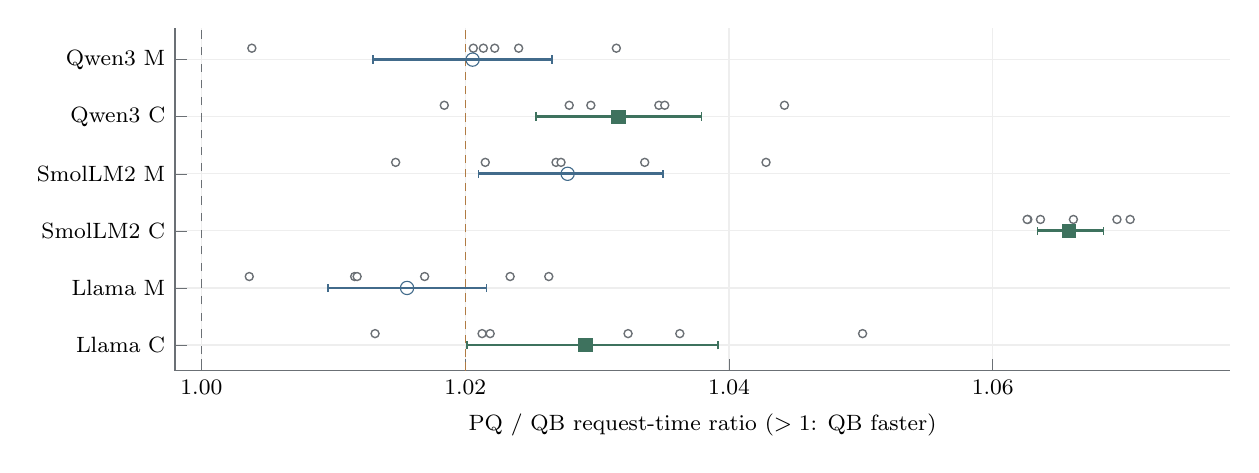
\begin{tikzpicture}[font=\footnotesize]
\begin{axis}[name=sess,scale only axis,width=13.4cm,height=4.35cm,
xmin=.998,xmax=1.078,xtick={1,1.02,1.04,1.06},xticklabels={1.00,1.02,1.04,1.06},
ymin=.55,ymax=6.55,ytick={6,5,4,3,2,1},yticklabels={Qwen3 M,Qwen3 C,SmolLM2 M,SmolLM2 C,Llama M,Llama C},
xlabel={PQ / QB request-time ratio ($>1$: QB faster)},xlabel style={font=\footnotesize},tick label style={font=\footnotesize},
axis lines*=left,axis line style={aux},tick style={aux},grid=major,grid style={gray!13}]
\draw[aux,dashed] (axis cs:1,.55)--(axis cs:1,6.55);
\draw[draft,densely dashed] (axis cs:1.02,.55)--(axis cs:1.02,6.55);
\addplot[only marks,mark=*,mark size=1.45pt,mark options={draw=aux,fill=white,line width=.5pt},color=aux] coordinates {(1.022241155,6.2) (1.003825879,6.2) (1.024056173,6.2) (1.031462696,6.2) (1.020617513,6.2) (1.021379783,6.2)};
\addplot[only marks,mark=*,mark size=1.45pt,mark options={draw=aux,fill=white,line width=.5pt},color=aux] coordinates {(1.018417206,5.2) (1.034686907,5.2) (1.029528424,5.2) (1.027889260,5.2) (1.044209114,5.2) (1.035132037,5.2)};
\addplot[only marks,mark=*,mark size=1.45pt,mark options={draw=aux,fill=white,line width=.5pt},color=aux] coordinates {(1.021523343,4.2) (1.042811401,4.2) (1.026887696,4.2) (1.027267920,4.2) (1.014728654,4.2) (1.033614105,4.2)};
\addplot[only marks,mark=*,mark size=1.45pt,mark options={draw=aux,fill=white,line width=.5pt},color=aux] coordinates {(1.062659839,3.2) (1.069420131,3.2) (1.066117550,3.2) (1.070418529,3.2) (1.063618892,3.2) (1.062610884,3.2)};
\addplot[only marks,mark=*,mark size=1.45pt,mark options={draw=aux,fill=white,line width=.5pt},color=aux] coordinates {(1.011619881,2.2) (1.003629727,2.2) (1.026339325,2.2) (1.016926078,2.2) (1.023407939,2.2) (1.011808397,2.2)};
\addplot[only marks,mark=*,mark size=1.45pt,mark options={draw=aux,fill=white,line width=.5pt},color=aux] coordinates {(1.013167868,1.2) (1.050133956,1.2) (1.021893776,1.2) (1.036275997,1.2) (1.032350688,1.2) (1.021280772,1.2)};
% Asymmetric percentile intervals and point estimates are generated from the frozen table.
\draw[target,line width=1pt] (axis cs:1.013022800003,6)--(axis cs:1.026553489035,6);
\draw[target,line width=.65pt] (axis cs:1.013022800003,5.925)--(axis cs:1.013022800003,6.075);
\draw[target,line width=.65pt] (axis cs:1.026553489035,5.925)--(axis cs:1.026553489035,6.075);
\addplot[only marks,mark=o,mark size=2.4pt,target] coordinates {(1.020563161899,6)};
\draw[qualified,line width=1pt] (axis cs:1.025392736138,5)--(axis cs:1.037925690306,5);
\draw[qualified,line width=.65pt] (axis cs:1.025392736138,4.925)--(axis cs:1.025392736138,5.075);
\draw[qualified,line width=.65pt] (axis cs:1.037925690306,4.925)--(axis cs:1.037925690306,5.075);
\addplot[only marks,mark=square*,mark size=2.4pt,qualified] coordinates {(1.031613690048,5)};
\draw[target,line width=1pt] (axis cs:1.021009792824,4)--(axis cs:1.035016679387,4);
\draw[target,line width=.65pt] (axis cs:1.021009792824,3.925)--(axis cs:1.021009792824,4.075);
\draw[target,line width=.65pt] (axis cs:1.035016679387,3.925)--(axis cs:1.035016679387,4.075);
\addplot[only marks,mark=o,mark size=2.4pt,target] coordinates {(1.027767425686,4)};
\draw[qualified,line width=1pt] (axis cs:1.063387048182,3)--(axis cs:1.068398798323,3);
\draw[qualified,line width=.65pt] (axis cs:1.063387048182,2.925)--(axis cs:1.063387048182,3.075);
\draw[qualified,line width=.65pt] (axis cs:1.068398798323,2.925)--(axis cs:1.068398798323,3.075);
\addplot[only marks,mark=square*,mark size=2.4pt,qualified] coordinates {(1.065803002589,3)};
\draw[target,line width=1pt] (axis cs:1.009627059351,2)--(axis cs:1.021621860041,2);
\draw[target,line width=.65pt] (axis cs:1.009627059351,1.925)--(axis cs:1.009627059351,2.075);
\draw[target,line width=.65pt] (axis cs:1.021621860041,1.925)--(axis cs:1.021621860041,2.075);
\addplot[only marks,mark=o,mark size=2.4pt,target] coordinates {(1.015593036909,2)};
\draw[qualified,line width=1pt] (axis cs:1.020125595877,1)--(axis cs:1.039148610748,1);
\draw[qualified,line width=.65pt] (axis cs:1.020125595877,0.925)--(axis cs:1.020125595877,1.075);
\draw[qualified,line width=.65pt] (axis cs:1.039148610748,0.925)--(axis cs:1.039148610748,1.075);
\addplot[only marks,mark=square*,mark size=2.4pt,qualified] coordinates {(1.029113522487,1)};
\end{axis}
\end{tikzpicture}

\caption{Independent-block E2 replication. Small marks are the six session estimates; large markers and horizontal bars are the equal-weight estimate and its registered 95\% six-session percentile interval. Dashed lines mark parity and the 1.02 practical threshold. $M$ is target-only and $C$ speculative. The fixed exposed panel and single host limit statistical scope.}
\label{fig:e2}
\end{figure*}

All 36 family/path/session contrasts favor QB; 9 of the 72 family/path/task aggregates regress. The primary pointwise speculative intervals are [1.025393,1.037926], [1.063387,1.068399] and [1.020126,1.039149], each above the predeclared 1.02 threshold under the registered percentile method. Target-only effects are smaller: Llama's estimate is 1.015593, below the threshold, while Qwen3's interval overlaps it.

The secondary $t_5$ intervals remain above 1.02 for speculative Qwen3 and SmolLM2. Llama's interval is [1.015387,1.043026], above parity but crossing 1.02; its six leave-one-session-out estimates range from 1.024960 to 1.032333. QB's advantage is stable in these checks. Whether the Llama effect exceeds the practical threshold depends on the interval method. \sref{supp:cuda} reports both analyses and all task regressions.

E2 establishes endpoint and recorded-counter correspondence across all 216 speculative PQ/QB task/session pairs: acceptance, rollback and logical-workload counters agree. This supports an implementation-cost comparison under matched recorded work. The original two-session estimates and their target-only direction reversals are reported in \sref{supp:cost}; E2's recorded-counter scope is detailed in \sref{supp:cuda}.

The recovered E2 records do not report actual CUDA Graph capture, replay or fallback counts. The request-cost estimate therefore identifies the implementation effect but does not isolate those mechanisms. The controlled QB/QH replay study in Section~\ref{sec:mappingcosts} has its own execution evidence and comparator.


\subsection{Same-input correspondence across layers and phases}
\label{sec:numeric}
The initial 24-context replay established PQ/QB correspondence at sampled layer-0 attention boundaries. E1 expands the test to three layer positions, prefill and continuation, and $q=1,2,3,4$ in each family. All 72 contexts pass observation, native-MQ own-path and repeatability checks. PQ and QB are bitwise equal at QK, softmax and AV in every context, with zero maximum error and ULP distance (Figure~\ref{fig:numeric}).

\begin{figure}[t]\centering
\resizebox{\columnwidth}{!}{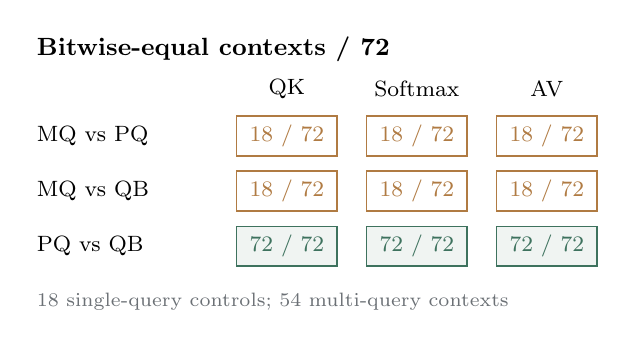
\begin{tikzpicture}[x=1cm,y=1cm,font=\footnotesize]
\node[anchor=west,font=\bfseries\small] at (0,2.65) {Bitwise-equal contexts / 72};
\foreach \x/\t in {3.30/QK,4.95/Softmax,6.60/AV}\node at (\x,2.15) {\t};
\foreach \y/\t in {1.55/MQ vs PQ,.85/MQ vs QB,.15/PQ vs QB}\node[anchor=west] at (0,\y) {\t};
\foreach \y in {1.55,.85}{\foreach \x in {3.30,4.95,6.60}{
 \draw[draft,line width=.65pt] (\x-.64,\y-.25) rectangle (\x+.64,\y+.25);
 \node[text=draft] at (\x,\y) {18 / 72};}}
\foreach \x in {3.30,4.95,6.60}{\draw[qualified,line width=.65pt,fill=qualified!8] (\x-.64,-.10) rectangle (\x+.64,.40);\node[text=qualified] at (\x,.15) {72 / 72};}
\node[anchor=west,text=aux,font=\scriptsize] at (0,-.55) {18 single-query controls; 54 multi-query contexts};
\end{tikzpicture}
}
\caption{Completed 72-context CUDA replay. The 18 agreements between MQ and either repair are exactly the $q=1$ common-path controls. The 54 multi-query cases first differ at QK. All PQ/QB stage outputs agree bitwise.}
\label{fig:numeric}
\end{figure}

The sampled target layers are $0/18/35$ for Qwen3, $0/12/23$ for SmolLM2 and $0/16/31$ for Llama. Qwen3 and Llama use head dimension 128 with 32 query heads and 8 KV heads; SmolLM2 uses dimension 64 with 32/32 heads. Thus the observed correspondence spans both ordinary and grouped-query attention and more than one head dimension.

MQ agrees with either repaired path only in the 18 single-query controls. Across the other 54 contexts, its first difference is at QK; maximum finite absolute differences are 0.078583 at QK, 0.000917 at softmax and 0.010433 at AV. These are operator differences on identical operands, not model-logit bounds.

All snapshots have tensor key extent 256, including masked padding. The maximum number of visible keys is 109, 130 and 127 by family; prefill captures include early query positions with only one to four visible keys. The experiment covers layers, phases and query widths at these short visible contexts, using one exposed prompt per family. Complete coordinates and operator comparisons appear in \sref{supp:cuda}.


\subsection{Matched deployment: k3 gains survive fresh contexts}
\label{sec:matchedbridge}
A new matched study separates the effects of speculative depth and context lifecycle within one runtime~\cite{rtxnativebridge}. It uses the original twelve exposed Qwen3 inputs, unchanged model/tokenizer bytes, context1024, target UB4, draft UB1 and cap128/native EOG. One executable supplies all four $k=1,3$ by resident/fresh cells and the PQ\_A/PQ\_B/QB arms. All 204 qualification requests preserve complete outputs and speculative state; corresponding PQ/QB decision vectors agree, and every output also matches the historical E2 reference.

Six independently loaded process sessions complete 864 measurements and 72 warmups. The order balances cells and arms within input/session blocks. Both models remain loaded. Resident requests clear their existing contexts; fresh requests create and destroy contexts inside the service timer. The shared timer includes prefill, generation, sampling, synchronization and result construction. Heavy capture and additional backend counters are disabled.

\begin{table*}[t]\centering\small
\caption{Matched Qwen3 deployment bridge. Ratios compare QB with the arithmetic mean of identical PQ controls; aggregation gives equal weight to inputs and process sessions. Intervals are the registered Bonferroni-adjusted session-bootstrap intervals for the four-cell family. The practical screen also requires reduction above the A/A threshold and improvement in every session.}
\label{tab:nativebridge}
\begin{tabular}{@{}rlll@{}}\toprule
$k$ & Lifecycle & QB/dual-PQ [simultaneous interval] & Practical gain\\\midrule
1 & Resident & 0.986617 [0.965043, 1.006956] & Not established\\
3 & Resident & 0.937404 [0.922603, 0.949354] & Established\\
1 & Fresh & 0.973534 [0.955904, 0.996512] & Not established\\
3 & Fresh & 0.946409 [0.940517, 0.953312] & Established\\
\bottomrule\end{tabular}
\end{table*}


QB reduces service time by 6.26\% at resident $k=3$ and 5.36\% at fresh $k=3$ (Table~\ref{tab:nativebridge}). Both pass the registered practical screen; neither $k=1$ cell passes. The $k=3$ point reductions exceed their respective 4.125\% and 4.388\% input-aggregate A/A imbalances and favor QB in every session. The four primary intervals resample whole process sessions and use a Bonferroni adjustment; the twelve inputs remain a fixed panel.

The layout benefit therefore survives fresh-context service at $k=3$. Secondary paired contrasts favor a stronger layout effect at $k=3$ in both lifecycles, while each individual lifecycle contrast includes parity. Changing $k$ changes the speculative transaction as well as query width. These comparisons identify a deployment-dependent layout effect, not a pure width intervention or a CUDA Graph mechanism. The new driver also does not reconstruct every difference between the older HTTP E2 and fresh-service contracts.

\subsection{Transfer to previously unexposed inputs}
\label{sec:transfer}
A separate study retains the three-family $k=3$ resident HTTP contract and tests twelve previously unexposed natural inputs per family~\cite{rtxtransferrecords}. The frozen panel covers formatted prompt-length strata 64--192, 256--448 and 640--832 within context1024. Short inputs are GSM8K mathematics; longer inputs are CodeContests code. Length and domain therefore vary together.

\begin{table*}[t]\centering\small
\caption{Transfer to previously unexposed inputs within context1024. Each family has a registered 12-input panel. Qwen3 and SmolLM2 complete all inputs; the Llama reference failure stops that family before cost measurement. The layout screen uses a 2\% floor, input-aggregate A/A and every-session direction; no population interval is assigned.}
\label{tab:heldouttransfer}
\begin{tabular}{@{}llll@{}}\toprule
Family & Reference qualification & QB/dual-PQ (screen) & QB/R\\\midrule
Qwen3 & 12/12 inputs pass & 0.967781 (not established) & 0.560577\\
SmolLM2 & 12/12 inputs pass & 0.930056 (pass) & 1.007007\\
Llama & PQ and QB both depart from R & Not run & Not run\\
\bottomrule\end{tabular}
\end{table*}


Qwen3 and SmolLM2 pass all twelve inputs. Four sessions per family supply 384 measurements and 384 warmups in total. SmolLM2's 6.99\% QB layout reduction passes the finite-panel practical screen, yet QB/R is 1.007007: the complete speculative request remains slightly slower than its serial reference. Qwen3's 3.22\% reduction is smaller than its 4.78\% A/A threshold. Layout value and profitable speculation remain separate questions.

Llama provides a reference-transfer counterexample. On CodeContests/valid/108, with 737 formatted prompt tokens, PQ and QB agree with each other in outputs, full decision vectors and causal trace, but both depart from deployed R at zero-based output index81. The remaining three Llama inputs and all Llama timing slots stay unexecuted. PQ/QB correspondence therefore does not establish reference preservation on a new input. The tested native-fast comparator also fails reference qualification in all three families; no qualified timing victory over that route is claimed. \sref{supp:followup} gives accounting and source access.

\subsection{Fresh-context request service}
\label{sec:service}
\subsubsection{Service and reference contracts}
The service studies integrate mapped verification into real speculative transactions and charge complete service cost. Both use a Qwen3-8B Q8\_0 target, Qwen3-0.6B Q8\_0 draft, four exposed inputs, $k=1$, F16 KV and non-flash attention. The platform panels have different formatting, output windows, frontends and prefill policies~\cite{b570servicerecords,rtxservicerecords}.

The timer spans fresh-context creation, graph reservation, prefill, generation, sampling, state handling, synchronization and context destruction. It includes host logits copies and native state work; correctness comparisons and raw-file output follow the timer. Shared model loading is recorded separately, and both models remain resident for target-only $R$. This window charges more lifecycle work than the resident HTTP requests in Section~\ref{sec:e2}.

For input $i$ and process session $s$, define the identical-PQ control mean and layout ratio
\begin{equation}
\bar T_{is,\PQ}=\tfrac12(T_{is,\PQ_A}+T_{is,\PQ_B}),\qquad
r_{is}=T_{is,\QB}/\bar T_{is,\PQ}.
\label{eq:servicepair}
\end{equation}
We aggregate $r_{is}$ geometrically with equal input and session weights; values below one favor QB. Separately, $d_{is}=T_{is,\QB}/T_{is,R}$ measures the frozen speculative policy's net value. The registered practical screen requires qualified outputs, a reduction above both 2\% and the largest absolute input-aggregate PQ\_A/PQ\_B imbalance, and a QB advantage in every session. All registered blocks enter this engineering screen.

\subsubsection{Vulkan: qualified requests, costly speculation}
The B570 bridge integrates the scoped GQA repair into a private model graph builder. Each fresh context fixes its layout before graph creation. Real-request traces record proposals, acceptance/correction/bonus decisions and KV trimming, and verify $q=2$, key256/512 and 32/8 GQA across all 36 target layers.

On HumanEval/38, /65, /115 and /127 with cap64 and natural EOG, R/PQ/QB endpoints agree. PQ/QB match 346 full-logit pairs, including rejected rows, and complete cycle traces. Four timing processes perform 64 measurements and 16 separately recorded warmups. QB/dual-PQ is 0.995144: its 0.486\% point reduction falls below the 2\% practical margin. The largest input-aggregate A/A imbalance is 0.754\%. QB/R is 2.619763; speculation increases service cost under this policy~\cite{b570servicerecords}.

The mean target-verification host interval falls from 1.009015 to 0.935009 seconds (7.33\%), while draft prefill/decode costs 12.366798 seconds per QB request. These are host phase intervals. Changing the draft CPU-thread parameter from 8 to 1 preserves all 346 vectors but yields DRAFT1/dual-baseline 1.003994. One-task embedding operations may already clamp the effective worker count, so this parameter intervention neither improves cost nor identifies its physical cause~\cite{b570policyrecords}.

\subsubsection{RTX: useful speculation, unresolved layout increment}
The RTX study freezes a new driver and prospective full-logit reference, retaining model/tokenizer bytes, cap128 and 21 numerical DLLs. Independent R/PQ references preserve historical endpoints. QB matches PQ verification and draft vectors, including discarded rows, and the full cycle/state trace. Qualification omits operator readbacks that would split the CUDA graph. Metadata verifies caller $q=2$, QB physical $q=2$, PQ serial $q=1$ and all 36 layers~\cite{rtxservicerecords}.

Four fresh processes execute 64 measured requests and 64 separately charged warmups. Endpoint/state checks pass; all 16 paired blocks remain in the analysis. QB/dual-PQ is 0.989284, a 1.072\% point reduction, against 5.208\% maximum input-aggregate A/A imbalance; two of four sessions favor PQ. The practical QB increment remains unresolved, and the registered rule stops additional profiling.

QB/R is 0.582325, a 41.8\% service-time reduction, with all 16 paired ratios below one. Dual-PQ/R is already 0.588633 (Figure~\ref{fig:servicepanels}): most of this policy gain is obtained by PQ. R uses target UB1; speculation uses target UB4 and draft UB1. These frozen-policy comparisons separate profitable speculation from QB's unresolved additional value.

\begin{figure*}[t]
\centering\begin{tikzpicture}
\begin{groupplot}[group style={group size=3 by 1,horizontal sep=.68cm},
width=.305\textwidth,height=6.1cm,ymin=.5,ymax=2.65,ytick={1,2},
tick label style={font=\footnotesize},title style={font=\small},label style={font=\footnotesize,align=center},
axis lines*=left,axis line style={aux,line width=.45pt},tick style={aux},
grid=major,grid style={gray!12},clip=false]
\nextgroupplot[title={\textbf{A} Layout increment},xlabel={$T_{\QB}/\bar T_{\PQ}$\\$<1$: QB faster},xmin=.82,xmax=1.18,xtick={.85,1,1.15},yticklabels={B570,RTX}]
\addplot[aux,dashed,line width=.65pt] coordinates {(1,.5)(1,2.65)};
\addplot[aux,densely dotted] coordinates {(.98,.5)(.98,2.65)};
\addplot[only marks,mark=o,mark size=1.3pt,mark options={draw=qualified,fill=white,line width=.5pt},qualified] coordinates {(1.139826244244,1.790) (0.945849532204,1.817) (0.923908031504,1.844) (0.922589990337,1.871) (1.037840796194,1.898) (1.060687483585,1.925) (0.964678996272,1.952) (1.095850644734,1.979) (0.867051748054,2.006) (1.075364022151,2.033) (1.063243809835,2.060) (1.031135431587,2.087) (0.929089961795,2.114) (0.942869964094,2.141) (0.910151770722,2.168) (0.965631764151,2.195)};
\addplot[only marks,mark=diamond*,mark size=2.8pt,qualified] coordinates {(0.989283832162,2)};
\node[font=\footnotesize,text=qualified,anchor=south] at (axis cs:0.989283832162,2.23){0.9893};
\addplot[only marks,mark=o,mark size=1.3pt,mark options={draw=qualified,fill=white,line width=.5pt},qualified] coordinates {(0.994434518096,0.790) (0.994346955730,0.817) (0.997636159223,0.844) (0.998559725528,0.871) (0.995388158443,0.898) (0.990654252807,0.925) (0.997896355971,0.952) (0.997327956447,0.979) (0.997377153779,1.006) (0.992338895142,1.033) (0.996575875826,1.060) (0.998197853655,1.087) (0.991359732503,1.114) (0.990675696924,1.141) (0.997016709214,1.168) (0.992578048127,1.195)};
\addplot[only marks,mark=diamond*,mark size=2.8pt,qualified] coordinates {(0.995143975812,1)};
\node[font=\footnotesize,text=qualified,anchor=south] at (axis cs:0.995143975812,1.23){0.9951};
\nextgroupplot[title={\textbf{B} Identical-PQ control},xlabel={$T_{\PQ_A}/T_{\PQ_B}$\\identical implementation},xmin=.80,xmax=1.18,xtick={.85,1,1.15},yticklabels={,}]
\addplot[aux,dashed,line width=.65pt] coordinates {(1,.5)(1,2.65)};
\addplot[aux,densely dotted] coordinates {(.98,.5)(.98,2.65)};
\addplot[aux,densely dotted] coordinates {(1.02,.5)(1.02,2.65)};
\addplot[only marks,mark=o,mark size=1.3pt,mark options={draw=target,fill=white,line width=.5pt},target] coordinates {(0.995683567795,1.790) (0.948687206972,1.817) (1.002893498473,1.844) (0.937857123081,1.871) (1.018199057240,1.898) (0.928511175631,1.925) (1.133151458846,1.952) (0.908678851591,1.979) (0.836859699631,2.006) (0.996816614475,2.033) (0.950265018054,2.060) (1.012025769051,2.087) (0.951652309469,2.114) (0.953906893171,2.141) (0.890919556111,2.168) (1.005416311802,2.195)};
\addplot[only marks,mark=diamond*,mark size=2.8pt,target] coordinates {(0.964859750025,2)};
\node[font=\scriptsize,text=aux,anchor=south] at (axis cs:0.99,2.24){max. task imbalance 5.21\%};
\addplot[only marks,mark=o,mark size=1.3pt,mark options={draw=target,fill=white,line width=.5pt},target] coordinates {(1.000263373246,0.790) (0.998378236952,0.817) (0.999694644835,0.844) (1.001035132081,0.871) (0.997047068817,0.898) (1.001825902924,0.925) (1.000688705872,0.952) (0.998169208021,0.979) (1.001209202542,1.006) (0.997665280704,1.033) (0.998639552710,1.060) (0.998604248688,1.087) (0.999614281800,1.114) (0.992960821525,1.141) (1.000503281379,1.168) (0.972323667784,1.195)};
\addplot[only marks,mark=diamond*,mark size=2.8pt,target] coordinates {(0.997390415137,1)};
\node[font=\scriptsize,text=aux,anchor=south] at (axis cs:0.99,1.24){max. task imbalance 0.75\%};
\nextgroupplot[title={\textbf{C} Value of drafting},xlabel={Service / $T_R$ (log scale)\\$<1$: speculation faster},xmode=log,log basis x=10,xmin=.44,xmax=3.45,xtick={.5,1,2,3},xticklabels={0.5,1,2,3},yticklabels={,}]
\addplot[aux,dashed,line width=.65pt] coordinates {(1,.5)(1,2.65)};
\addplot[only marks,mark=o,mark size=1.1pt,mark options={draw=qualified,fill=white,line width=.45pt},qualified] coordinates {(0.860709500935,2.090) (0.626760614714,2.103) (0.620301508760,2.116) (0.536318432454,2.129) (0.605208924945,2.142) (0.598746155267,2.155) (0.643792756015,2.168) (0.587714386461,2.181) (0.507935515395,2.194) (0.574851260097,2.207) (0.656442531287,2.220) (0.530408922715,2.233) (0.516897971637,2.246) (0.519814743067,2.259) (0.528263723757,2.272) (0.492411464129,2.285)};
\addplot[only marks,mark=diamond*,mark size=2.5pt,qualified] coordinates {(0.582325110976,2.190)};
\node[font=\scriptsize,text=qualified,anchor=south] at (axis cs:0.582325110976,2.300){QB 0.5823};
\addplot[only marks,mark=o,mark size=1.1pt,mark options={draw=target,fill=white,line width=.45pt},target] coordinates {(0.755123428050,1.720) (0.662643045616,1.733) (0.671388804522,1.746) (0.581318286640,1.759) (0.583142353976,1.772) (0.564488753316,1.785) (0.667364748795,1.798) (0.536308838513,1.811) (0.585819146937,1.824) (0.534564341243,1.837) (0.617396052735,1.850) (0.514393072401,1.863) (0.556348677623,1.876) (0.551311170004,1.889) (0.580412784714,1.902) (0.509937102744,1.915)};
\addplot[only marks,mark=square*,mark size=2.5pt,target] coordinates {(0.588633001010,1.820)};
\node[font=\scriptsize,text=target,anchor=south] at (axis cs:0.588633001010,1.930){PQ 0.5886};
\addplot[only marks,mark=o,mark size=1.1pt,mark options={draw=qualified,fill=white,line width=.45pt},qualified] coordinates {(2.594995842505,1.090) (2.670002306074,1.103) (2.622363844693,1.116) (2.603504205863,1.129) (2.601387062271,1.142) (2.645054922828,1.155) (2.619781081148,1.168) (2.604889445075,1.181) (2.602635519004,1.194) (2.647093847080,1.207) (2.619384718054,1.220) (2.602523908884,1.233) (2.592298609216,1.246) (2.645997993711,1.259) (2.617612598821,1.272) (2.628099334862,1.285)};
\addplot[only marks,mark=diamond*,mark size=2.5pt,qualified] coordinates {(2.619762936381,1.190)};
\node[font=\scriptsize,text=qualified,anchor=south] at (axis cs:2.619762936381,1.300){QB 2.6198};
\addplot[only marks,mark=o,mark size=1.1pt,mark options={draw=target,fill=white,line width=.45pt},target] coordinates {(2.609519073689,0.720) (2.685181757420,0.733) (2.628577383096,0.746) (2.607259374984,0.759) (2.613439832700,0.772) (2.670008143944,0.785) (2.625303785781,0.798) (2.611868471385,0.811) (2.609479783192,0.824) (2.667530074694,0.837) (2.628384633415,0.850) (2.607222505392,0.863) (2.614891975358,0.876) (2.670902296209,0.889) (2.625445064894,0.902) (2.647750813975,0.915)};
\addplot[only marks,mark=square*,mark size=2.5pt,target] coordinates {(2.632546646573,0.820)};
\node[font=\scriptsize,text=target,anchor=south] at (axis cs:2.632546646573,0.930){PQ 2.6325};
\end{groupplot}
\end{tikzpicture}

\caption{Service costs under separate platform contracts. Small outlined points show all 16 input/session blocks per contrast; large markers are equal-weight geometric means. A: QB/dual-PQ. B: identical-PQ A/A, with the largest absolute input-aggregate imbalance used by the screen. C: both speculative paths relative to target-only R. Dashed lines mark parity; dotted lines show 2\%. Vertical offsets separate observations. Ratios below one favor the numerator. The platform panels are analyzed separately.}
\label{fig:servicepanels}
\end{figure*}

The positive $k=3$ resident-request result and unresolved $k=1$ service increment use different drivers, inputs and cost windows. Their difference identifies a deployment question, not an isolated context-creation effect. \sref{supp:service} gives complete blocks, identities and incomplete follow-ups.

\section{Transferring a local repair}
\label{sec:state}
\begin{figure*}[t]\centering
\resizebox{\textwidth}{!}{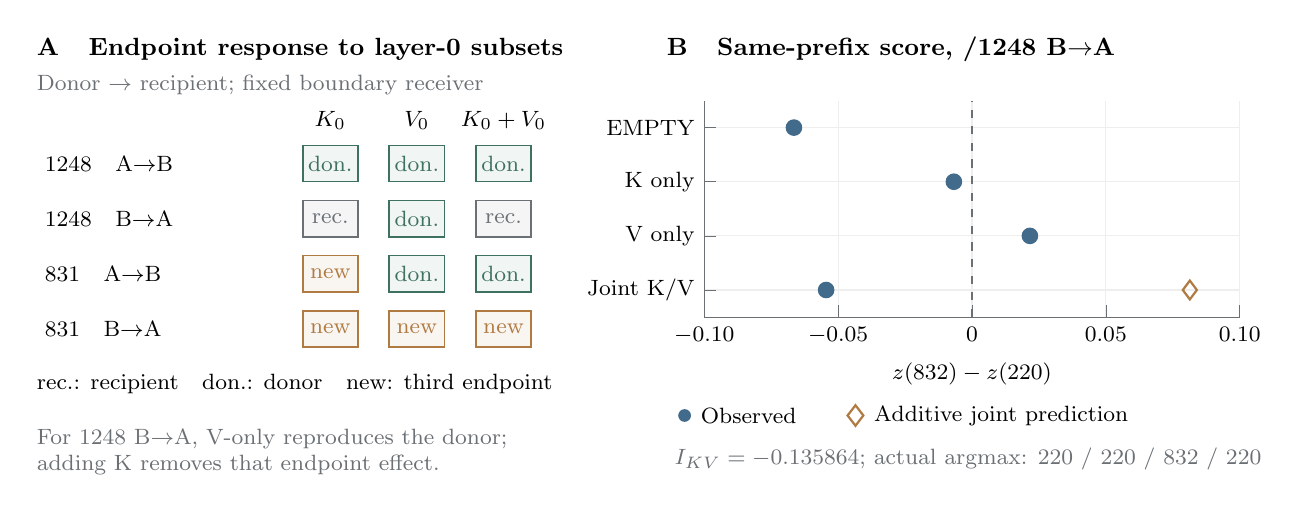
\begin{tikzpicture}[font=\footnotesize,x=1cm,y=1cm]
\node[anchor=west,font=\small\bfseries] at (0,4.4) {A\quad Endpoint response to layer-0 subsets};
\node[anchor=west,text=aux] at (0,3.95) {Donor $\to$ recipient; fixed boundary receiver};
\node at (3.85,3.5) {$K_0$};\node at (4.95,3.5) {$V_0$};\node at (6.05,3.5) {$K_0+V_0$};
\foreach \y/\lab in {2.95/{1248\quad A$\to$B},2.25/{1248\quad B$\to$A},1.55/{831\quad A$\to$B},.85/{831\quad B$\to$A}} {
 \node[anchor=west] at (.1,\y) {\lab};}
\foreach \x/\y/\v/\col in {3.85/2.95/B/qualified,4.95/2.95/B/qualified,6.05/2.95/B/qualified,3.85/2.25/D/aux,4.95/2.25/B/qualified,6.05/2.25/D/aux,3.85/1.55/C/draft,4.95/1.55/B/qualified,6.05/1.55/B/qualified,3.85/.85/C/draft,4.95/.85/C/draft,6.05/.85/C/draft}{
 \draw[\col,fill=\col!7,line width=.6pt] (\x-.35,\y-.23) rectangle ++(.7,.46);
 \if\v D\def\endpoint{rec.}\else\if\v B\def\endpoint{don.}\else\def\endpoint{new}\fi\fi
 \node[text=\col] at (\x,\y) {\endpoint};}
\node[anchor=west] at (0,.15) {rec.: recipient\quad don.: donor\quad new: third endpoint};
\node[anchor=north west,align=left,text=aux] at (0,-.3) {For 1248 B$\to$A, V-only reproduces the donor;\\adding K removes that endpoint effect.};
\node[anchor=west,font=\small\bfseries] at (8.0,4.4) {B\quad Same-prefix score, /1248 B$\to$A};
\begin{axis}[at={(8.6cm,1cm)},anchor=south west,scale only axis,width=6.8cm,height=2.75cm,
xmin=-.10,xmax=.10,xtick={-.10,-.05,0,.05,.10},xticklabels={$-0.10$,$-0.05$,0,0.05,0.10},
ymin=.5,ymax=4.5,ytick={4,3,2,1},yticklabels={EMPTY,K only,V only,Joint K/V},
axis lines*=left,axis line style={aux},tick style={aux},tick label style={font=\footnotesize},
xlabel={$z(832)-z(220)$},xlabel style={font=\footnotesize},grid=major,grid style={gray!13}]
\draw[aux,dashed] (axis cs:0,.5)--(axis cs:0,4.5);
\addplot[only marks,mark=*,mark size=2.8pt,target] coordinates {(-.06651496887207031,4)(-.006771087646484375,3)(.021633148193359375,2)(-.05448722839355469,1)};
\addplot[only marks,mark=diamond,mark size=3.4pt,draft,line width=.8pt] coordinates {(.08137702941894531,1)};
\end{axis}
\fill[target] (8.35,-.25) circle[radius=2.3pt];
\node[anchor=west,inner sep=0pt] at (8.55,-.25) {Observed};
\draw[draft,line width=.8pt] (10.42,-.25)--(10.52,-.12)--(10.62,-.25)--(10.52,-.38)--cycle;
\node[anchor=west,inner sep=0pt] at (10.75,-.25) {Additive joint prediction};
\node[anchor=west,text=aux] at (8.1,-.8) {$I_{KV}=-0.135864$; actual argmax: 220 / 220 / 832 / 220};
\end{tikzpicture}
}
\caption{State composition at two levels. A: layer-0 endpoint classes; rec. retains the recipient, don. reproduces a distinguishable donor and new is a third trajectory. Each cell has two agreeing process repeats. B: full-logit comparison for /1248, B$\to$A, at output 47 after a common consumed prefix. The hollow diamond is the additive prediction, not a fifth execution.}
\label{fig:composition}
\end{figure*}

\subsection{Qualify the producer state}
A local attention repair consumes state produced upstream. The B570 studies test whether prefill partitioning changes that state and the resulting single-query continuation. With target context UB512 and output capacity one, arm A submits the whole prompt; B splits it into 128 tokens and a remainder. Arm C uses UB128 with internal partitioning. All arms request final-position logits and then continue naturally.

For two exposed inputs of 161 and 133 prompt tokens, B reproduces C's complete endpoint, initial FP32 logits and sequence-KV bytes. A diverges at generated indices 47 and 81. Two longer controls have unequal A/B states but equal endpoints. A partition sweep yields several endpoint classes, including a third trajectory for the 133-token input split as $132+1$: smaller chunks are not monotonically closer to the reference (\sref{supp:b570}).

The differences begin before attention: first-layer K/V projections differ for the 161-token input, and Q/K/V differ for the 133-token input. Fixed-operand replay qualifies 32 of 40 calls and reproduces projection sensitivity. Eight scale/MUL calls are excluded because an in-place consumer overwrote their captured operands. The partition sweep's driver-body preregistration gap and replay admission record are retained in \sref{supp:b570}.

A common UB512 receiver isolates the state link. It imports sequence KV and positions, samples the selected complete initial logits, and restores pending-token semantics. Sixteen own-path shams reproduce natural endpoints; 40 crosses then vary KV and logit sources. For the two affected tasks,
\begin{align}
Y(KV_A,L_A)=Y(KV_A,L_B)&=Y_A,\\
Y(KV_B,L_A)=Y(KV_B,L_B)&=Y_B.
\label{eq:cross}
\end{align}
All initial vectors choose token 1271, making the logit swap a first-decision negative control. The suffix follows the KV source; the stable controls retain their endpoint despite unequal KV. Local consumer qualification alone cannot certify the producer state. Transfer requires qualification of both.

\subsection{Endpoint agreement and state substitution}
\label{sec:composition}
The subset study tests ten selectors on four exposed inputs in both donor directions. After 32 EMPTY/ALL controls, 80 coordinates each run in two independent processes, with agreement at every coordinate. Of the 160 requests, 30 reproduce a distinguishable donor endpoint, 54 produce a third trajectory and 76 retain the recipient endpoint despite changed bytes (\sref{supp:composition}).

A layer-0 K-only or V-only replacement selects $1/64$ of total K/V value storage and can reproduce a donor endpoint. This sufficiency is nonmonotone. For /1248 B$\to$A, layer-0 V reproduces the donor, but adding K removes that effect. In the reverse direction, layer-0 V works while replacing V at every layer does not.

Endpoint equality also fails as a cache-substitution criterion. Natural A/B states for /1011 and /1249 have equal endpoints but unequal KV. On /1011, 16 of 20 subset/direction coordinates produce a third trajectory; all 20 retain the endpoint on /1249. These interventions refute arbitrary component interchangeability; they do not establish natural reachability of mixed states.

To distinguish additive changes crossing an argmax threshold from a nonadditive score response, we compare full FP32 logits at the first divergence after a common consumed prefix. For fixed tokens $(r,u)$, write $d_S=z_S(u)-z_S(r)$ and
\begin{equation}
I_{KV}=d_{KV}-d_K-d_V+d_\emptyset.
\label{eq:interaction}
\end{equation}
For /1248 B$\to$A at output 47, $(r,u)=(220,832)$. EMPTY/K/V/KV scores are $-0.066515$, $-0.006771$, $+0.021633$ and $-0.054487$. The additive prediction is $+0.081377$, opposite in sign to the observed joint score; $I_{KV}=-0.135864$. Full-vocabulary argmax tokens are 220/220/832/220. The result establishes a nonadditive response through subsequent computation, without localizing it to one kernel.

\sref{supp:composition} records the 44 complete contrasts among 112 planned repeat-level contrasts, canonical token coordinates and missing vectors.

\subsection{Qualify backend execution}
\label{sec:backend}
The original Vulkan pilot combines reference-like or bulk prefill with MQ, PQ or QB continuation. Reference monitoring fails the declared sampling schedule: 48 of 49 attempted requests complete, one is interrupted and 31 coordinates remain unstarted. Speculative QB also changes the /831 and /1011 outputs. The pilot fails qualification; \sref{supp:pilot} retains its full record.

Independent address and scalar oracles pass 432 synthetic fixtures over 72 geometries. Yet the original $q=2$ QB graph violates a necessary condition of the frozen Vulkan matrix-multiplication backend:
\begin{equation}
b_3(\mathrm{src}_0)=b_3(\mathrm{src}_1),
\label{eq:backend}
\end{equation}
where $b_3$ is the fourth tensor extent. QK pairs K at extent 1 with lifted Q at extent 2; AV pairs V at extent 1 with probabilities at extent 2. Both are rejected. MQ and each PQ slice satisfy this check with $(1,1)$.

This is a version-specific source admission result. Actual placement and fallback transfers were not observed in the failed pilot. The checker records the proven violation as false and the remaining admission decisions as unknown.

\subsection{Preserving the AV path in a scoped GQA port}
A scoped port targets F16/F32, $d=128$, 32-query-head/8-KV-head layouts, physical key extents 256/512 and $q=2,4$. Its packed route matches PQ at QK and softmax but differs in 7,160 of 8,192 AV values at key512/$q=2$, with maximum absolute difference $1.22236\times10^{-9}$. That route fails the exact reference~\cite{b570gqarecords}.

The successful route reuses the existing noncontiguous AV shader with zero V batch stride, real probability/output strides and independent query workgroups. All six key256/512 by $q=1,2,4$ coordinates match byte-for-byte at QK, softmax, AV and final output; all 20 earlier PQ stage files remain unchanged. The port retains per-output evaluation while exposing parallel work across queries. Section~\ref{sec:service} qualifies this fixed-layout port in real requests; the earlier Llama Q6\_K pilot remains failed.

\section{From layout cost to service cost}
\label{sec:mappingcosts}
\subsection{Mapping execution and representation costs}
\subsubsection{Execution mode changes the comparison}
We compare PQ, QB and query-to-head mapping (QH), which places independent queries in a head-like dimension and then restores native output order. Each operator study freezes its inputs, reference and cost window~\cite{mappingrecords,b570compactrecords}.

Graph allocations initially reused K/V storage and changed later operands. Independent persistent storage restored repeatable input and output bytes. Balanced experiments then used identical QB arms to measure A/A variation. On the RTX core panel, QB\_A/QH is 0.900826. A frozen selector predicts the ordering on 12 held-out synthetic geometries, but charging its lookup raises the offline estimated selector/fixed-QB ratio to 1.010298. Selection overhead outweighs the predicted benefit.

CUDA Graph capture, instantiation and replay materially change the relative costs. QB\_A's completed-graph ON/OFF ratios range from 0.615 to 0.849. For four permuted-$q=2$ coordinates, the QH-minus-QB gap falls from 12.056--12.975 to 0.735--1.627\,$\mu$s. Instrumented mode checks and clean timing runs share frozen graph/runtime identities. This intervention identifies an execution-mode effect on QB versus QH; it does not measure the PQ/QB mechanism in the resident-request study.

\subsubsection{Path availability and reference preservation}
RTX key extents 1023/1024/1025 select 8/3/8-kernel paths, with completed graph-replay costs of 113.085/50.439/114.618\,$\mu$s. To separate physical extent from logical visibility, a padding intervention fixes each input and original mask columns, then appends finite zero K/V and fully masked columns~\cite{mappingrecords}.

Padding logical length 1023 to physical extent 1024 reaches the three-kernel path on the first call but fails the unpadded reference on all four qualification hosts. Padding to 1025 passes all four, retains eight kernels and costs about 1.5\% more than either native QB control. The faster path is therefore available but inadmissible under the frozen reference (Figure~\ref{fig:mappingboundary}); it has no qualified steady-state cost.

\begin{figure*}[t]
\centering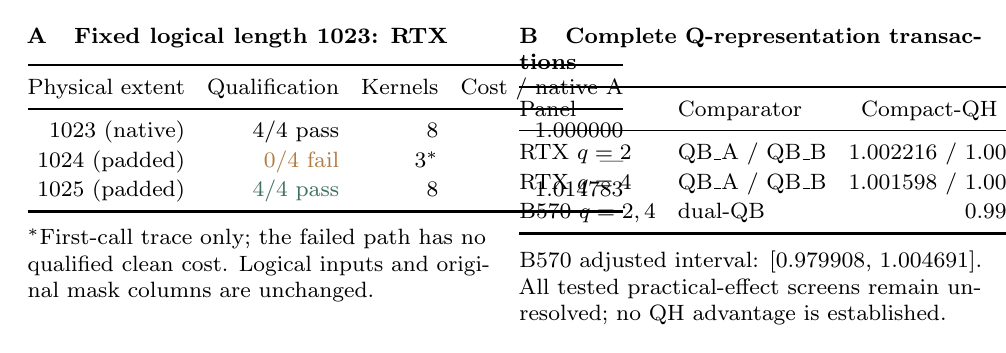
\begin{tikzpicture}[font=\footnotesize]
\node[anchor=north west,inner sep=0] at (0,0) {\begin{minipage}[t]{.48\textwidth}
\textbf{A\quad Fixed logical length 1023: RTX}\par\vspace{5pt}
\begin{tabular}{@{}rrrr@{}}\toprule
Physical extent & Qualification & Kernels & Cost / native A\\\midrule
1023 (native) & 4/4 pass & 8 & 1.000000\\
1024 (padded) & \textcolor{draft}{0/4 fail} & 3$^\ast$ & ---\\
1025 (padded) & \textcolor{qualified}{4/4 pass} & 8 & 1.014783\\\bottomrule
\end{tabular}\par\vspace{5pt}
$^\ast$First-call trace only; the failed path has no qualified clean cost. Logical inputs and original mask columns are unchanged.
\end{minipage}};
\node[anchor=north west,inner sep=0] at (.515\textwidth,0) {\begin{minipage}[t]{.48\textwidth}
\textbf{B\quad Complete Q-representation transactions}\par\vspace{5pt}
\begin{tabular}{@{}llr@{}}\toprule
Panel & Comparator & Compact-QH ratio\\\midrule
RTX $q=2$ & QB\_A / QB\_B & 1.002216 / 1.008295\\
RTX $q=4$ & QB\_A / QB\_B & 1.001598 / 1.004167\\
B570 $q=2,4$ & dual-QB & 0.992244\\\bottomrule
\end{tabular}\par\vspace{5pt}
B570 adjusted interval: [0.979908, 1.004691]. All tested practical-effect screens remain unresolved; no QH advantage is established.
\end{minipage}};
\end{tikzpicture}

\caption{Reference and transaction constraints on mapping optimization. A: the length-1023 padding candidate reaches a three-kernel path on its first call but fails the reference. B: complete Q-representation transactions with explicit comparators. RTX and B570 use different geometries and execution modes. The B570 interval is descriptive and family-adjusted.}
\label{fig:mappingboundary}
\end{figure*}

\subsubsection{Charging the representation transaction}
Compact Q removes a QH graph copy but must first be produced. The RTX timer covers the continuous transaction from common permuted host Q through copy/transpose, upload, graph replay/synchronization and complete ordinary-output readback. K/V and mask are resident; targets are preallocated. The window excludes model Q production and ongoing KV updates.

For $q=2$ and $q=4$, compact-QH/QB\_A transaction ratios are 1.002216 and 1.001598; relative to QB\_B they are 1.008295 and 1.004167. Neither passes the practical screen against both controls. The B570 equal-head study likewise establishes no practical QH benefit: compact-QH/dual-QB is 0.992244, with descriptive adjusted interval [0.979908,1.004691] and paired difference $-1.518\,\mu$s [$-4.168,+0.916$]. \sref{supp:followupmapping} retains the separate resident-graph results.

Fixed QB remains the baseline in these domains: a representation must repay its production and consumption costs, not just reduce internal graph work.

\section{A deployment decision rule}
\label{sec:decisionrule}
The results support an ordered comparison of qualified implementations.

\paragraph{Choose the repair scope before judging the draft.}
For each repair organization, compare target-only and speculative requests under the same reference, inputs and timer. The seven-arm experiment shows that this choice changes the sign of draft value for two families. A draft rejected under global serialization can be profitable after local repair; a draft paired with a faster layout can still lose to target-only execution. Qualification must cover the intended inputs: the later Llama counterexample shows that mutually agreeing PQ/QB executions can both depart from the deployed reference~\cite{rtxtransferrecords}.

\paragraph{Preserve evaluation within a query and expose work across queries.}
The Q/mask views preserve logical operands and indexing. The scoped Vulkan port supplies the backend counterpart: retain the noncontiguous AV shader, use a zero V batch stride and dispatch independent query workgroups~\cite{b570gqarecords}. Its packed alternative loses byte correspondence. Phase/layout tags and producer-state qualification are therefore part of the interface, alongside tensor shapes and strides. Endpoint equality alone does not license cache-component substitution.

\paragraph{Charge the complete deployment transaction.}
After selecting local repair, compare QB directly with PQ. Include graph preparation, reuse, submission and request lifecycle costs in the intended service window. The common-runtime bridge establishes a practical QB benefit at $k=3$ for both resident and fresh contexts, while neither $k=1$ cell passes the screen~\cite{rtxnativebridge}. Draft length changes the measured value of the layout; fresh-context overhead does not by itself eliminate that value. The B570 prefill-submission follow-up supplies a separate negative result: reducing API submissions preserves the reference but does not clear the service-benefit screen~\cite{b570prefillrecords}. Select the cheaper qualified policy using the complete request, not acceptance rate, caller count or one operator interval alone.

These control points complement batch-invariant kernels~\cite{thinkingmachines}, reproducible accumulation~\cite{reproblas} and phase-aware tiled execution~\cite{spectra}. A hardware extension must preserve the declared evaluation, including matrix-instruction details beyond dtype~\cite{ptx}, and beat an equal-resource baseline at a measured request-critical cost. The archived same-policy AV model supplies a parity control, not that performance evidence~\cite{studyrecords}.

\section{Related work and evidence scope}
\label{sec:related}
\subsection{Where numerical consistency is enforced}
Query-axis parallelism is established attention structure. FlashAttention uses tiled attention to reduce memory traffic~\cite{flashattention}; FlashAttention-2 distributes query rows across thread blocks and warps while sharing K/V~\cite{flashattention2}. These methods optimize fused evaluation and work partitioning. QB instead expresses independent queries through views of existing non-flash operators and integrates their one-query organization with phase selection, graph reuse and speculative state. Its qualification target is the output of a specified deployed numerical stack.

Table~\ref{tab:relatedmechanisms} compares the closest control points. Batch-invariant inference stabilizes reductions in normalization, matrix multiplication and attention~\cite{thinkingmachines}. CoRun combines isolated prefill, fixed-shape decode and selective kernel constraints~\cite{corun}. LLM-42 runs a fast path, verifies fixed-shape windows and repairs the corresponding KV entries~\cite{llm42}. These systems define reproducible execution contracts; matching an already deployed quantized reference is a separate requirement.

\begin{table*}[t]\centering\small
\caption{Numerical-consistency control points. Performance comparisons in this paper use GS and PQ in the same runtime.}\label{tab:relatedmechanisms}
\begin{tabularx}{\textwidth}{@{}>{\raggedright\arraybackslash}p{2.3cm}>{\raggedright\arraybackslash}p{3.3cm}YY@{}}\toprule
Approach & Consistency target & Constraint and arithmetic & State and verification\\\midrule
Batch-invariant kernels~\cite{thinkingmachines}
& Each token's result is invariant to batching and slicing
& Stable reduction/tiling rules in kernels, including attention split size
& Consistent KV layout before attention; no added verify--rollback loop\\
CoRun~\cite{corun}
& Stable token sequence across co-runners, batch positions and arrival orders in a fixed stack
& Isolated prefill and fixed-shape CUDA-Graph decode; disable decode Split-KV and constrain collectives
& Request-local cache and RNG state; shape control supplies the execution contract\\
LLM-42~\cite{llm42}
& Tokens agree with a fixed-shape verification schedule
& Dynamic fast path plus fixed-shape replay; mostly existing kernels
& Verify--rollback and replacement of decoded KV entries by verified entries\\
Phase-scoped QB
& Complete output agrees with the specified ordinary reference on the qualified panel
& Q/mask views preserve local one-query attention; surrounding computation remains batched
& Phase/layout-aware reuse, producer-state qualification and native speculative reconciliation\\\bottomrule
\end{tabularx}
\end{table*}

QB's method is the integrated graph/runtime transformation. It reuses attention operators while changing query/mask representation, preserving head semantics and binding the layout to phases and graph identity. The Vulkan AV-preserving port shows that backend admission can still require an implementation change. Local numerical correspondence and stateful endpoint qualification test different parts of this contract.

Other approaches act at different boundaries. LayerCast separates storage and computation precision~\cite{layercast}; TBIK aligns reductions across tensor-parallel configurations~\cite{tbik}; MarginGate selects verification using decision margins~\cite{margingate}. Vosti specifies engine/kernel behavior across batching, chunking and cache changes and proves guarantees under its assumptions~\cite{vosti}. Our logical mapping proof, runtime guards, operator replay and endpoint tests supply finite qualification against the specified reference.

\subsection{State and request cost}
Stage-Replay demonstrates suffix sensitivity to KV transplantation~\cite{stagereplay}, and cache-dependent divergence is reported in quantized serving~\cite{cachestate}. Our fixed-precision interventions add component-substitution counterexamples and common-prefix score comparisons. Activation-patching studies establish the importance of intervention metrics and nonadditive component effects~\cite{patching,mediators}; our four-cell score contrast tests nonadditivity beyond an endpoint pattern caused only by thresholding.

Ragged-batch synchronization errors supply a separate source of speculative failures~\cite{forensics}. We check semantic indexing, finite-precision correspondence and backend admission separately. Work on verification cost and actual execution behavior~\cite{illusion,lossless} also motivates complete-request measurement. Our matched comparisons add the repair--draft interaction and isolate QB's incremental cost relative to PQ.

\subsection{Scope of the empirical results}
The CUDA request results cover one sequence, non-flash attention, $q\leq4$, Q8\_0 weights, F16 KV and context1024. E2 estimates variation across six sessions on one host for a fixed 12-input panel; E1 samples one prompt per family at physical key extent 256 and short visible contexts. The new-input study extends formatted prompts to 811 tokens and observed continuation visibility to 938 keys. Its short mathematical and longer programming inputs vary domain and length together~\cite{rtxtransferrecords}. The Llama counterexample in Section~\ref{sec:transfer} bounds reference transfer. All three families reject the tested native-fast comparator, so qualified cost comparisons remain against the declared serial and repaired paths.

The Vulkan state interventions concern four exposed inputs and finite greedy continuations. The stopped Llama Q6\_K pilot remains unqualified. The Qwen3 Q8\_0 port has its own reference and runtime; native replay covers four complete requests, a real layer-0/key512/$q=2$ fixture and its first-query $q=1$ slice~\cite{b570nativereproduction}. The historical $k=1$ service and prefill-submission screens, including the latter's incomplete helper-process accounting, are retained in \sref{supp:service}.

The matched Qwen3 study estimates a joint draft-length/lifecycle contrast on twelve exposed inputs. Its six process sessions occur on one date; the four cluster-bootstrap intervals have nominal family coverage and quantify process-session variation on that host~\cite{rtxnativebridge}. Individual lifecycle contrasts include parity. The service estimates include the full declared request window, while CUDA Graph capture/replay mechanisms and the remaining differences between historical drivers are unidentified. Contexts beyond 1024, concurrent throughput, energy and hardware efficiency are unmeasured. Native rebuild/replay establishes source-host execution; external access to bulk tensors and pinned numerical dependencies is specified separately from saved-data reconstruction and CPU checks in \sref{supp:reproduction}.

\section{Conclusion}
\label{sec:conclusion}
Phase-scoped QB offers a concrete way to constrain attention query geometry while retaining surrounding target batching. The original CUDA studies establish bitwise PQ/QB attention correspondence on a fixed replay and lower complete-request cost on the registered three-family panel. Later mapping experiments show that execution mode, reference admissibility and representation preparation constrain how far that local result can be optimized.

The newer B570 and RTX request panels add an important distinction. Both qualify real q=2 execution and preserve the registered endpoints and state traces, yet neither establishes a practical QB-over-PQ layout gain under its predeclared screen. Their speculative economics differ: the RTX policy is faster than target-only on its finite exposed panel, whereas the B570 policy is substantially more expensive. These are bounded results under different runtime contracts, not a cross-device ranking.

The evidence justifies an empirical architecture discussion about reference-preserving graph transformations, backend support and complete cost accounting. It does not yet justify a new accelerator design. A hardware direction should follow only if a measurable request-critical residual survives the strongest qualified software baseline and can be tied to a concrete physical mechanism.

\section*{Data and code availability}
The manuscript package includes reported data, analysis scripts, editable figures and CPU interface tests. Companion repositories provide native build/replay kits and small real fixtures. RTX rebuilds the core/frontend with pinned numerical binaries; B570 rebuilds its numerical libraries and shaders. Full request references and some pinned dependencies remain on the source hosts. \sref{supp:reproduction} and \texttt{REPRODUCTION\_ACCESS.md} identify the versioned materials, external dependencies and remaining delivery steps.
\section*{Declaration of AI-assisted work}
OpenAI ChatGPT and Codex assisted implementation, analysis code, figures and writing. Measurements come from recorded executions. The author is responsible for verifying the results, interpretations and references and approving the final text.
\balance
\setlength{\bibsep}{0pt plus .1pt minus .1pt}
\bibliographystyle{psql-num}
\bibliography{references}
\clearpage
\nobalance
\setcounter{section}{0}
\setcounter{table}{0}
\setcounter{figure}{0}
\setcounter{equation}{0}
\renewcommand{\thesection}{S\arabic{section}}
\renewcommand{\thetable}{S\arabic{table}}
\renewcommand{\thefigure}{S\arabic{figure}}
\renewcommand{\theequation}{S\arabic{equation}}
\renewcommand{\theHsection}{supp.\arabic{section}}
\renewcommand{\theHtable}{supp.\arabic{table}}
\renewcommand{\theHfigure}{supp.\arabic{figure}}
\renewcommand{\theHequation}{supp.\arabic{equation}}
\twocolumn[{
\phantomsection\label{supp:start}
\pdfbookmark[0]{Supplementary material}{supplement-title}
\begin{center}
{\Large\bfseries Supplementary material}\par\vspace{5pt}
{\normalsize Phase-Scoped Query Layouts for Reference-Preserving Speculative Decoding}
\end{center}
\noindent Complete comparison tables and reproduction details. Section, figure, table and equation numbers use an S prefix; pages and citations continue from the article. Development history and detailed audit logs are indexed in the ancillary files.\par\vspace{7pt}
\noindent\small\hyperref[supp:implementation]{S1: implementation}\quad
\hyperref[supp:confirmation]{S2--S3: CUDA evidence}\quad
\hyperref[supp:b570]{S4--S6: Vulkan evidence}\quad
\hyperref[supp:followupmapping]{S7--S8: follow-up studies}\quad\hyperref[supp:reproduction]{S9: reproduction}\par
\vspace{9pt}\hrule\vspace{11pt}
}]

\section{Implementation and reference contracts}
\label{supp:implementation}\label{supp:contracts}
The CUDA target/draft pairs use Q8\_0 conversions and F16 KV; the original B570 state-study target uses Q6\_K and the historical draft Q4\_K\_M. Model families, converted files and reference recipes remain distinct between campaigns. Native endpoint checks retain IDs, EOG flags, length, last token and stop reason. Older first-EOG or re-tokenized-text comparisons have their original scope in the ancillary history; they do not qualify newer full-array comparisons.

\subsection{Implementation checks}
Query views must fit the allocated source span, preserve alignment and nonoverlapping logical coordinates, and maintain the original mask column and GQA mapping. K/V ownership and the output permutation are checked explicitly. The role/phase flag enters graph parameters before the observation-disabled branch, participates in topology reuse and resets on a new request. PQ slices identical operands and masks; GS actually changes physical target microbatching. Neither baseline changes the draft, reconciliation or stopping rule to create a cost difference.

\subsection{Complete phase-selection experiment}
The four-bit experiment tests four HumanEval probes, two repeats, $k=3$, UB4 and cap128: 128 native requests. Table~\ref{tab:masks} preserves every mask. Mask3 is inclusion-minimal within this tested family and is fixed in the later campaigns. A separate 19-task/six-repeat comparison against all-phase mask15 gave only 1.003569 generation speed, below its registered 1.03 threshold, with an interval including parity. Removing constraints was not itself an established efficiency improvement.
\begin{table}[t]\centering\small
\setlength{\tabcolsep}{2.8pt}
\caption{Historical finite four-switch pattern. TP/TC/DP/DC are target/draft prefill/continuation bits. ``Y'' means full-reference match on that probe in the tested repeats.}
\label{tab:masks}
\begin{tabular}{@{}rccccccccc@{}}\toprule
Mask&TP&TC&DP&DC&HE15&HE18&HE25&HE31&Panel\\\midrule
0&0&0&0&0&Y&N&N&Y&N\\
1&1&0&0&0&Y&N&Y&Y&N\\
2&0&1&0&0&Y&N&Y&Y&N\\
3&1&1&0&0&Y&Y&Y&Y&Y\\
4&0&0&1&0&Y&N&N&Y&N\\
5&1&0&1&0&Y&N&Y&Y&N\\
6&0&1&1&0&Y&N&Y&Y&N\\
7&1&1&1&0&Y&Y&Y&Y&Y\\
8&0&0&0&1&Y&N&N&Y&N\\
9&1&0&0&1&Y&N&Y&Y&N\\
10&0&1&0&1&Y&N&Y&Y&N\\
11&1&1&0&1&Y&Y&Y&Y&Y\\
12&0&0&1&1&Y&N&N&Y&N\\
13&1&0&1&1&Y&N&Y&Y&N\\
14&0&1&1&1&Y&N&Y&Y&N\\
15&1&1&1&1&Y&Y&Y&Y&Y\\\bottomrule
\end{tabular}
\end{table}
\subsection{Width and runtime boundaries}
The earlier joint $(k,U)$ sweep tested $(1,2),(3,4),(5,6),(7,8)$ at caps 128/256/512 on 11 inputs. MBPP229 failed in the two wider geometries; a separate HumanEval18 failure retained its own denominator. The maximum observed reference length was 261, so requesting cap512 did not establish a 512-token complete trajectory. In a fixed-UB4 study, widening $k$ to 7 preserved endpoints but yielded generation/request ratios of 0.829442/0.889868 versus $k=3$. Draft proposals increased from 3,528 to 5,392 while accepted draft tokens increased from 2,772 to 3,192. Different captured sessions showed caller counts falling from 305 to 199 and micrographs rising from 305 to 397; these are not additive component timings.

Four engineering PQ warm requests failed when graph metadata capacity was insufficient. A resource-only correction scaled metadata reservation by the already declared maximum $q=4$ without changing numerical operators or the formal panel. SmolLM2/Llama PQ arms use that registered executable; the other arms retain the original route with identical numerical DLLs. Alias-admission and packaging corrections remain in the archive. They are not additional scientific replications.

\section{Complete output and repair-cost results}
\label{supp:confirmation}\label{supp:cost}
\subsection{Larger confirmation}
The larger campaign has 3,600 complete required requests: three families, five arms, 24 tasks, two adjacent sessions and five repetitions, plus 150 excluded warmups. Its panel was frozen against accessible execution history. $M_3$ and $C_3$ each match 240/240 endpoints per family. $M_0$ differs on 5, 14 and 9 tasks; the Qwen3 failures are GSM8K141,443,562,660,722. The ordinary-production path qualifies for Qwen3 but fails 140 SmolLM2 and 80 Llama requests. Table~\ref{tab:largecost} keeps failed comparisons as dashes.
\begin{table}[t]\centering\small
\caption{Larger confirmation ratios. Numerator time / denominator time. Dashes preserve failed qualification.}
\label{tab:largecost}
\label{tab:confirmationratios}
\begin{tabular}{@{}lrrr@{}}\toprule
Comparison&Qwen3&SmolLM2&Llama\\\midrule
$R_{\rm prod}/C_3$&1.569566&---&---\\
$M_3/C_3$&1.134924&0.607389&1.072227\\
$R/C_3$&1.569977&0.877174&1.609468\\
$M_0/M_3$&---&---&---\\
$R/M_0$&---&---&---\\
$R/M_3$&1.383332&1.444173&1.501051\\
$R_{\rm prod}/M_3$&1.382970&---&---\\\bottomrule
\end{tabular}
\end{table}
For $M_3/C_3$, regressed tasks number 0/24, 24/24 and 4/24. Llama regressions are MBPP418,476,79,99. Failed $M_0/M_3$ comparisons have diagnostic ratios 0.968456, 0.948603 and 0.936943; failed SmolLM2/Llama $R_{\rm prod}/C_3$ comparisons are 0.512333 and 0.842790. They remain unqualified because the outputs differ. The 72 separate lite timing observations did not establish mutually exclusive completed GPU stages; their component model remains unavailable.

\subsection{Seven-arm implementation comparison}
The 12-task panel comprises MBPP 123, 140, 255, 401, 413, 418 and GSM8K 111, 120, 1308, 141, 322, 443. Two adjacent sessions and four repetitions per arm/family give 2,016 formal requests and 96 qualified endpoints per arm/family. Table~\ref{tab:allcost} gives all 21 ratios. Figure~\ref{fig:taskcost} retains the task-level local-repair and draft comparisons.
\begin{table}[t]\centering\small
\caption{All 21 qualified implementation comparisons at reported six-decimal precision. Regressions count tasks on which the denominator is slower.}
\label{tab:allcost}
\begin{tabular}{@{}llrr@{}}\toprule
Family&Comparison&Ratio&Regressions\\\midrule
Qwen3 & $M_{\PQ}/M_{\QB}$ & 1.026676 & 2/12 \\
Qwen3 & $C_{\PQ}/C_{\QB}$ & 1.043676 & 0/12 \\
Qwen3 & $M_{\GS}/M_{\QB}$ & 1.330106 & 0/12 \\
Qwen3 & $C_{\GS}/C_{\QB}$ & 2.143525 & 0/12 \\
Qwen3 & $M_{\QB}/C_{\QB}$ & 1.143749 & 1/12 \\
Qwen3 & $R/M_{\QB}$ & 1.334051 & 0/12 \\
Qwen3 & $R/C_{\QB}$ & 1.525820 & 0/12 \\
SmolLM2 & $M_{\PQ}/M_{\QB}$ & 1.038478 & 0/12 \\
SmolLM2 & $C_{\PQ}/C_{\QB}$ & 1.068111 & 0/12 \\
SmolLM2 & $M_{\GS}/M_{\QB}$ & 1.366008 & 0/12 \\
SmolLM2 & $C_{\GS}/C_{\QB}$ & 1.462530 & 0/12 \\
SmolLM2 & $M_{\QB}/C_{\QB}$ & 0.633948 & 12/12 \\
SmolLM2 & $R/M_{\QB}$ & 1.369890 & 0/12 \\
SmolLM2 & $R/C_{\QB}$ & 0.868439 & 10/12 \\
Llama & $M_{\PQ}/M_{\QB}$ & 1.013407 & 1/12 \\
Llama & $C_{\PQ}/C_{\QB}$ & 1.021848 & 2/12 \\
Llama & $M_{\GS}/M_{\QB}$ & 1.411508 & 0/12 \\
Llama & $C_{\GS}/C_{\QB}$ & 2.175941 & 0/12 \\
Llama & $M_{\QB}/C_{\QB}$ & 1.116620 & 1/12 \\
Llama & $R/M_{\QB}$ & 1.426161 & 0/12 \\
Llama & $R/C_{\QB}$ & 1.592480 & 0/12 \\
\bottomrule\end{tabular}
\end{table}
\begin{figure*}[t]\centering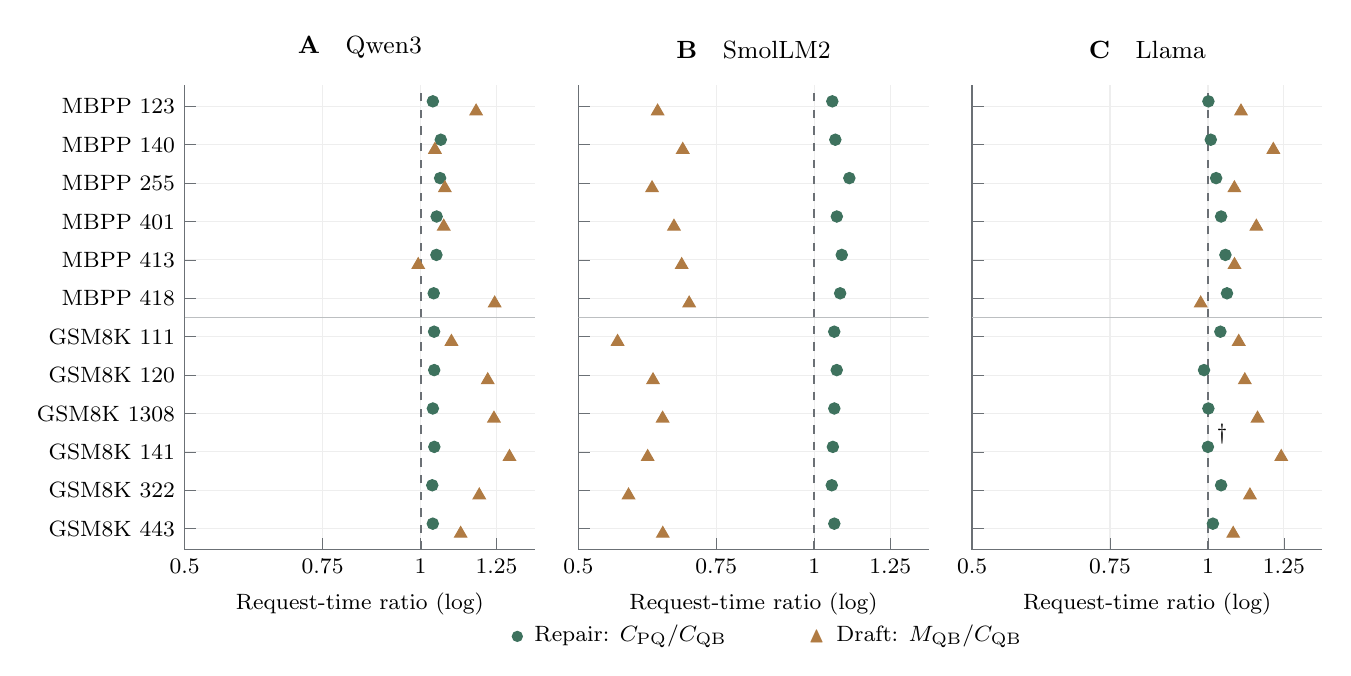
\begin{tikzpicture}[font=\footnotesize]
\pgfplotsset{tc/.style={scale only axis,width=4.45cm,height=5.9cm,
 xmin=.5,xmax=1.4,xtick={.5,.75,1,1.25},xticklabels={0.5,0.75,1,1.25},
 ymin=.45,ymax=12.55,ytick={12,11,10,9,8,7,6,5,4,3,2,1},
 tick label style={font=\footnotesize},title style={font=\small},
 xlabel={Request-time ratio (log)},xlabel style={font=\footnotesize},
 axis lines*=left,axis line style={aux,line width=.45pt},tick style={aux},grid=major,grid style={gray!13}}}
\begin{axis}[tc,xmode=log,log basis x=10,name=task0,title={\textbf{A}\quad Qwen3},yticklabels={{MBPP 123},{MBPP 140},{MBPP 255},{MBPP 401},{MBPP 413},{MBPP 418},{GSM8K 111},{GSM8K 120},{GSM8K 1308},{GSM8K 141},{GSM8K 322},{GSM8K 443}}]
\draw[aux!45,line width=.5pt] (axis cs:.5,6.5)--(axis cs:1.4,6.5);
\draw[aux,dashed,line width=.7pt] (axis cs:1,.45)--(axis cs:1,12.55);
\addplot[only marks,mark=*,mark size=2.05pt,qualified] coordinates {
(1.036885338768,12.13) % MBPP 123
(1.061278554900,11.13) % MBPP 140
(1.059180111967,10.13) % MBPP 255
(1.048438982047,9.13) % MBPP 401
(1.047751381369,8.13) % MBPP 413
(1.039442169125,7.13) % MBPP 418
(1.040676604660,6.13) % GSM8K 111
(1.040972953480,5.13) % GSM8K 120
(1.036854847813,4.13) % GSM8K 1308
(1.041304047650,3.13) % GSM8K 141
(1.035034462783,2.13) % GSM8K 322
(1.036689677369,1.13) % GSM8K 443
};
\addplot[only marks,mark=triangle*,mark size=2.55pt,draft] coordinates {
(1.177367374837,11.87) % MBPP 123
(1.043153552033,10.87) % MBPP 140
(1.074075758083,9.87) % MBPP 255
(1.070535881226,8.87) % MBPP 401
(0.993164444227,7.87) % MBPP 413
(1.243362773843,6.87) % MBPP 418
(1.095005490294,5.87) % GSM8K 111
(1.218256613173,4.87) % GSM8K 120
(1.240706906343,3.87) % GSM8K 1308
(1.298631817724,2.87) % GSM8K 141
(1.188324324823,1.87) % GSM8K 322
(1.125144610899,0.87) % GSM8K 443
};
\end{axis}
\begin{axis}[tc,xmode=log,log basis x=10,name=task1,title={\textbf{B}\quad SmolLM2},yticklabels={},at={(task0.east)},anchor=west,xshift=.55cm]
\draw[aux!45,line width=.5pt] (axis cs:.5,6.5)--(axis cs:1.4,6.5);
\draw[aux,dashed,line width=.7pt] (axis cs:1,.45)--(axis cs:1,12.55);
\addplot[only marks,mark=*,mark size=2.05pt,qualified] coordinates {
(1.054566083575,12.13) % MBPP 123
(1.063918529902,11.13) % MBPP 140
(1.108677458865,10.13) % MBPP 255
(1.068625097207,9.13) % MBPP 401
(1.084196407182,8.13) % MBPP 413
(1.079139647477,7.13) % MBPP 418
(1.060507704161,6.13) % GSM8K 111
(1.068385763399,5.13) % GSM8K 120
(1.060715564836,4.13) % GSM8K 1308
(1.056283852216,3.13) % GSM8K 141
(1.052871745769,2.13) % GSM8K 322
(1.060719024115,1.13) % GSM8K 443
};
\addplot[only marks,mark=triangle*,mark size=2.55pt,draft] coordinates {
(0.631103662893,11.87) % MBPP 123
(0.679553416367,10.87) % MBPP 140
(0.620910388381,9.87) % MBPP 255
(0.662221673125,8.87) % MBPP 401
(0.677409023433,7.87) % MBPP 413
(0.692464307030,6.87) % MBPP 418
(0.561083608097,5.87) % GSM8K 111
(0.622707419118,4.87) % GSM8K 120
(0.640490501227,3.87) % GSM8K 1308
(0.612980380488,2.87) % GSM8K 141
(0.579466032829,1.87) % GSM8K 322
(0.640824088900,0.87) % GSM8K 443
};
\end{axis}
\begin{axis}[tc,xmode=log,log basis x=10,name=task2,title={\textbf{C}\quad Llama},yticklabels={},at={(task1.east)},anchor=west,xshift=.55cm]
\draw[aux!45,line width=.5pt] (axis cs:.5,6.5)--(axis cs:1.4,6.5);
\draw[aux,dashed,line width=.7pt] (axis cs:1,.45)--(axis cs:1,12.55);
\addplot[only marks,mark=*,mark size=2.05pt,qualified] coordinates {
(1.001370147605,12.13) % MBPP 123
(1.008376337115,11.13) % MBPP 140
(1.024421134201,10.13) % MBPP 255
(1.039410861167,9.13) % MBPP 401
(1.052726772817,8.13) % MBPP 413
(1.057636679886,7.13) % MBPP 418
(1.037236647116,6.13) % GSM8K 111
(0.988542445882,5.13) % GSM8K 120
(1.001253575813,4.13) % GSM8K 1308
(0.999919059593,3.13) % GSM8K 141
(1.039432299111,2.13) % GSM8K 322
(1.014664677619,1.13) % GSM8K 443
};
\addplot[only marks,mark=triangle*,mark size=2.55pt,draft] coordinates {
(1.102019468994,11.87) % MBPP 123
(1.211831282673,10.87) % MBPP 140
(1.080833620771,9.87) % MBPP 255
(1.152939217798,8.87) % MBPP 401
(1.081181827097,7.87) % MBPP 413
(0.978890103612,6.87) % MBPP 418
(1.094724760208,5.87) % GSM8K 111
(1.114421752151,4.87) % GSM8K 120
(1.156852932560,3.87) % GSM8K 1308
(1.240381150408,2.87) % GSM8K 141
(1.131389453725,1.87) % GSM8K 322
(1.077053710346,0.87) % GSM8K 443
};
\node[anchor=south west,inner sep=0pt,xshift=3pt,yshift=1pt,font=\footnotesize] at (axis cs:0.999919059593,3.13) {$\dagger$};
\end{axis}
\coordinate (legend) at ($(task1.south)+(0,-1.10cm)$);
\fill[qualified] ($(legend)+(-3cm,0)$) circle[radius=2.05pt];
\node[anchor=west,inner sep=0pt,xshift=6pt] at ($(legend)+(-3cm,0)$) {Repair: $C_{\PQ}/C_{\QB}$};
\node[draft,inner sep=0pt] at ($(legend)+(.8cm,0)$) {$\blacktriangle$};
\node[anchor=west,inner sep=0pt,xshift=7pt] at ($(legend)+(.8cm,0)$) {Draft: $M_{\QB}/C_{\QB}$};
\end{tikzpicture}

\caption{Original repair campaign: task-level local-repair benefit $C_{\PQ}/C_{\QB}$ (circles) and draft increment $M_{\QB}/C_{\QB}$ (triangles). Session medians are combined geometrically. The dagger marks Llama GSM8K141, whose local-repair ratio is 0.999919. These are not E2 observations.}
\label{fig:taskcost}\end{figure*}

Qwen3 target-only local-repair regressions are GSM8K141 and 322. Llama regresses on MBPP418 for target-only and GSM8K120,141 for speculative local repair. SmolLM2 favors QB on all tasks in both local comparisons. Every GS/QB task favors QB. For the draft increment, Qwen3 regresses on MBPP413, Llama on MBPP418, and SmolLM2 on all 12 tasks. SmolLM2's ordinary-to-candidate comparison regresses on 10/12.

The original session-specific ratios are retained below. Target-only Qwen3 and Llama reverse direction; speculative comparisons favor QB in both adjacent sessions. E2 tests these small effects with a different, independently scheduled design and is reported separately.
\begin{table}[t]\centering\small
\caption{Original two-adjacent-session PQ/QB ratios.}\label{tab:oldsessions}
\begin{tabular}{llrr}\toprule
Family & Path & Session 0 & Session 1\\\midrule
Qwen3&M&0.971380&1.085118\\
Qwen3&C&1.041728&1.045626\\
SmolLM2&M&1.040019&1.036939\\
SmolLM2&C&1.066179&1.070046\\
Llama&M&0.994477&1.032698\\
Llama&C&1.016460&1.027264\\
\bottomrule\end{tabular}\end{table}
All original task-level and session values are retained in \texttt{anc/plot\_values.json}. The paired-ratio identities used for draft value assume the same complete panel and weights. They do not estimate attention, projection, feed-forward or synchronization shares of request time.

\section{RTX replication and numerical replay}
\label{supp:cuda}
\subsection{E2 design and complete estimates}
The replication retains the 12-task implementation panel and the original reference, models, sampler, timer and runtime routes. Each session has 54 fresh workers: short PQ/QB blocks and serial-reference blocks, with one registered warmup per worker. Across six sessions this gives 864 PQ/QB requests, 432 references and 324 warmups. Each task/session has two matching serial-reference endpoints. All required endpoints and observation checks pass; no latency is trimmed.

The fixed runtime routes use the original executable for every Qwen3 arm and all R/QB arms. SmolLM2 and Llama PQ arms use the recorded metadata4 correction; both builds retain identical hashes for all 21 numerical DLLs. The source/build manifests identify each route. The launcher clears inherited GGML/CUDA environment overrides, but neither that configuration nor GGML topology reuse establishes actual CUDA Graph replay. Per-request capture, replay and fallback counts are absent from the recovered E2 report records.

\texttt{E2\_REQUEST\_LATENCIES.csv} retains all 1,620 rows, including the 324 labelled warmups, with its original Git-blob identity. \texttt{generate\_e2\_absolute\_cost.py} checks the source and reconstructs Table~\ref{tab:e2absolute}. The per-arm geometric means use the same 12-task and six-session weights as Equation~\ref{eq:ratio}, so their quotients reproduce the paired ratios. The table's \texttt{latency\_ms} is the resident request interval; raw start/end nanosecond fields remain in the full request archive.

All consecutive session gaps exceed one hour; first-to-last start is 24.450801 hours. The original interpreter bytes were restored after a pre-start identity mismatch before the final session. The original freeze checks then passed without exception and the untouched scientific slots ran. The earlier stopped record remains part of the history.

Table~\ref{tab:e2full} gives the complete six-session estimates. The intervals use the original random seed 20261014, 10,000 bootstrap draws of six session log means, and linearly interpolated 2.5/97.5 percentiles. They quantify fixed-panel, single-host variation, not a date-level population or multiple-comparison guarantee. Table~\ref{tab:e2tasks} gives all 72 task aggregates; 9 regress. Full session contrasts and observed session times are in \texttt{anc/rtx104/}.
\begin{table*}[t]\centering\small
\caption{All completed E2 comparisons. Ratios favor QB above one; regressions count six-session task point estimates below one.}\label{tab:e2full}
\begin{tabular}{llrrrrl}\toprule
Family&Path&Ratio&Lower 95\%&Upper 95\%&Regressions&Practical threshold 1.02\\\midrule
Qwen3&M&1.020563&1.013023&1.026553&2/12&Point above; interval overlaps\\
Qwen3&C&1.031614&1.025393&1.037926&1/12&Interval above\\
SmolLM2&M&1.027767&1.021010&1.035017&2/12&Interval above\\
SmolLM2&C&1.065803&1.063387&1.068399&0/12&Interval above\\
Llama&M&1.015593&1.009627&1.021622&3/12&Point below; interval overlaps\\
Llama&C&1.029114&1.020126&1.039149&1/12&Interval above\\
\bottomrule\end{tabular}\end{table*}
\begin{table*}[t]\centering\small
\caption{E2 task-level PQ/QB ratios, geometrically averaged over six sessions. Values below one are italicized; these are descriptive task contrasts, not significance tests.}\label{tab:e2tasks}
\begin{tabular}{lrrrrrr}\toprule
&\multicolumn{2}{c}{Qwen3}&\multicolumn{2}{c}{SmolLM2}&\multicolumn{2}{c}{Llama}\\
\cmidrule(lr){2-3}\cmidrule(lr){4-5}\cmidrule(l){6-7}
Task & M & C & M & C & M & C\\\midrule
GSM8K 111&1.015305&1.028626&1.031259&1.064372&1.027335&1.029118\\
GSM8K 120&1.007356&1.073052&1.050246&1.073224&1.021427&1.026504\\
GSM8K 1308&1.018527&1.030064&1.057675&1.070511&1.020762&1.041848\\
GSM8K 141&\textit{0.992667}&1.035252&1.021013&1.051986&1.012332&1.028335\\
GSM8K 322&1.001169&1.033028&1.028420&1.059544&1.026791&\textit{0.993618}\\
GSM8K 443&1.003752&1.021251&1.033367&1.067165&1.024666&1.019558\\
MBPP 123&1.056908&1.037495&1.044148&1.058628&\textit{0.992752}&1.023365\\
MBPP 140&\textit{0.981806}&1.052058&1.041709&1.063535&\textit{0.978786}&1.048076\\
MBPP 255&1.079294&1.032638&\textit{0.972948}&1.090371&1.021555&1.054405\\
MBPP 401&1.001954&1.024979&1.044272&1.048708&1.026712&1.009394\\
MBPP 413&1.089971&\textit{0.967860}&\textit{0.978119}&1.089698&\textit{0.986121}&1.035206\\
MBPP 418&1.004440&1.046335&1.033875&1.052829&1.050112&1.041465\\
\bottomrule\end{tabular}\end{table*}

Recorded acceptance, rollback and logical-workload counters agree in all 216 speculative task/session pairs. This comparison is limited to the recorded counters and histograms, rather than complete control-trace identity. Model callers and physical micrographs remain distinct from hardware launches.

\subsection{Sensitivity to interval method and session omission}
The registered percentile bootstrap remains the primary analysis. Table~\ref{tab:e2sensitivity} adds a post-review $t$ interval,
\[
\exp\!\left(\bar z\pm t_{0.975,5}\frac{s_z}{\sqrt6}\right),
\qquad t_{0.975,5}=2.570581835636314,
\]
where $z_s$ is the session mean log contrast and $s_z$ its sample standard deviation. This analysis assumes independent, approximately normal session log means; it does not add inputs, dates or hosts. Six further point estimates omit one session each.

All speculative $t$ intervals remain above parity. Qwen3 and SmolLM2 also remain above the practical ratio threshold 1.02; Llama crosses it. Its omit-one estimates all exceed 1.02. Thus the direction of the Llama effect is stable across these checks, while its practical-threshold conclusion depends on the interval method. The source CSV is unchanged; \texttt{scripts/generate\_e2\_sensitivity.py} reconstructs the new table and the complete omit-one estimates.
\begin{table*}[t]\centering\small
\caption{E2 session sensitivity on the fixed 12-input panel. Ratios are PQ/QB; $M$ is target-only and $C$ is speculative. The registered bootstrap remains primary. Secondary $t_5$ intervals assume independent, approximately normal session log means. The final column gives the range of six leave-one-session-out point estimates.}\label{tab:e2sensitivity}
\begin{tabular}{@{}llrrrr@{}}\toprule
Family & Path & Estimate & Primary bootstrap 95\% CI & Secondary $t_5$ 95\% CI & Omit-one range\\\midrule
Qwen3 & $M$ & 1.020563 & [1.013023, 1.026553] & [1.011013, 1.030204] & [1.018397, 1.023944]\\
Qwen3 & $C$ & 1.031614 & [1.025393, 1.037926] & [1.022587, 1.040720] & [1.029113, 1.034273]\\
SmolLM2 & $M$ & 1.027767 & [1.021010, 1.035017] & [1.017648, 1.037987] & [1.024785, 1.030395]\\
SmolLM2 & $C$ & 1.065803 & [1.063387, 1.068399] & [1.062196, 1.069422] & [1.064882, 1.066443]\\
Llama & $M$ & 1.015593 & [1.009627, 1.021622] & [1.006830, 1.024433] & [1.013457, 1.018003]\\
Llama & $C$ & 1.029114 & [1.020126, 1.039149] & [1.015387, 1.043026] & [1.024960, 1.032333]\\
\bottomrule\end{tabular}
\end{table*}


\subsection{E1 coverage and controls}
The independently frozen diagnostic retains all 21 numerical DLLs and changes only the two admitted capture/replay source files. Its 72 contexts use target layers $0/\lfloor L/2\rfloor/(L-1)$, both phases and $q=1$--4. One exposed text, GSM8K443, is selected by longest inherited prompt with lexical tie-breaking for each tokenizer. It has 105/126/123 prompt IDs for Qwen3/SmolLM2/Llama. Each context has a fresh worker with a counts warmup, heavy capture and counts control; each observed MQ/PQ/QB graph is replayed twice. All 72 contexts are observed and admitted; all requests and 432 operator starts complete.

The physical key extent is 256 in every capture. The per-query visible mask counts are 1 through $q$ in prefill, 106 through $105+q$ for Qwen3 continuation, 127 through $126+q$ for SmolLM2, and 124 through $123+q$ for Llama. Minimum-key selectors refer to tensor extent, not unmasked context; this is not a query-width by visible-length factorial. All exact coordinates are in \texttt{E1\_CONTEXTS.csv}.

PQ/QB bitwise equality is 72/72 at each stage. MQ/PQ and MQ/QB equality is 18/72, exclusively the $q=1$ controls. Table~\ref{tab:e1errors} retains the largest measured differences. These compare operator arrays, not next-token logits.
\begin{table}[t]\centering\small
\caption{E1 maximum MQ-to-repair differences; both repairs give the same values. PQ/QB has zero error and ULP distance at all stages.}\label{tab:e1errors}
\begin{tabular}{lrr}\toprule
Stage&Max. finite absolute&Max. finite ULP\\\midrule
QK&0.078582763671875&2,017,357,824\\
Softmax&0.0009172558784484863&96,633\\
AV&0.010433197021484375&1,953,885,696\\\bottomrule
\end{tabular}\end{table}

Large ULP distances near zero or across signs are retained rather than converted into a tolerance-based pass. Input identity is checked before and after replay against frozen hashes. Native worker module receipts are retained; the inherited standalone replay binds executable and DLL paths but does not add a separate loaded-module inventory. Kernel symbols, reduction trees and continuous residency remain unidentified.

\subsection{Restoration and interpretation}
The host downloaded and restored the authenticated E2, E1 and control archives into a fresh directory, verifying 10,179, 9,696 and 47 members. A separate interpreter reconstructed 11 analysis outputs byte-for-byte. This is same-host restoration, not an external replication. This manuscript's own checker reconstructs the six ratios and bootstrap intervals from the submitted session table, verifies the copied context/time-table identities and checks the report summaries; it does not replay the original tensor archives.

\section{Vulkan partition and retained-state experiments}
\label{supp:b570}
\subsection{Inputs and partition controls}
A uses UB512/capacity one and a whole-prompt submission; B retains that context and externally submits $128+\mathrm{remainder}$; C uses UB128 with internal partitioning. Only the final absolute prompt position requests logits. Three repeats per input/arm, one capture-off and two capture-on, give 63 requests. All B/C initial full FP32 logits, source-defined sequence-KV payloads and complete endpoints agree.
\begin{table}[t]\centering\small
\setlength{\tabcolsep}{3.3pt}
\caption{Seven original partition inputs. All B/C full endpoints and initial FP32/KV payloads agree. The first difference is A/B, zero-based.}
\begin{tabular}{@{}lrrl@{}}\toprule
Input&Prompt IDs&First difference&A/B initial state\\\midrule
GSM1248&161&47&Different\\
GSM831&133&81&Different\\
GSM1011&190&---&Different\\
GSM1249&163&---&Different\\
Prefix 1248/127&127&---&Equal\\
Prefix 1248/128&128&---&Equal\\
Prefix 1248/129&129&57&Different\\\bottomrule
\end{tabular}
\end{table}
Initial state comprises 64 F16 K/V tensors over 32 layers and recorded logical positions. Full KV payloads are retained at prefill completion; later cuts contain full logits but only KV hashes. The synthetic prefix129 difference at 57 was not added retrospectively as a capture cut.

The final follow-up contains 21 fourth-arm observations, 38 partition-sweep observations, 18 native captures, 16 shams and 40 crosses: 133 whole requests, with a zero-forward load probe separately counted. All 19 schedules are listed in Table~\ref{tab:allpart}. Driver-body hashes were authenticated only after the fourth-arm and sweep stages, which remain diagnostic rather than fully compliant confirmation. Authentication preceded the operator and restoration stages.
\begin{table}[t]\centering\small
\caption{All frozen exposed partition schedules. The final column is first output difference from A; no numerical monotonicity is inferred.}
\label{tab:allpart}
\begin{tabular}{@{}lllr@{}}\toprule
Input&Caller widths&Endpoint class&First diff.\\\midrule
1248&64+64+33&A&---\\
1248&96+65&A&---\\
1248&128+33&B/C&47\\
1248&160+1&A&---\\
831&64+64+5&A&---\\
831&96+37&A&---\\
831&128+5&B/C&81\\
831&132+1&Third class&40\\
1011&64+64+62&All&---\\
1011&96+94&All&---\\
1011&128+62&All&---\\
1011&160+30&All&---\\
1249&64+64+35&All&---\\
1249&96+67&All&---\\
1249&128+35&All&---\\
1249&160+3&All&---\\
Prefix 129&64+65&A&---\\
Prefix 129&96+33&A&---\\
Prefix 129&128+1&B/C&57\\\bottomrule
\end{tabular}
\end{table}
\begin{figure}[t]\centering\resizebox{\columnwidth}{!}{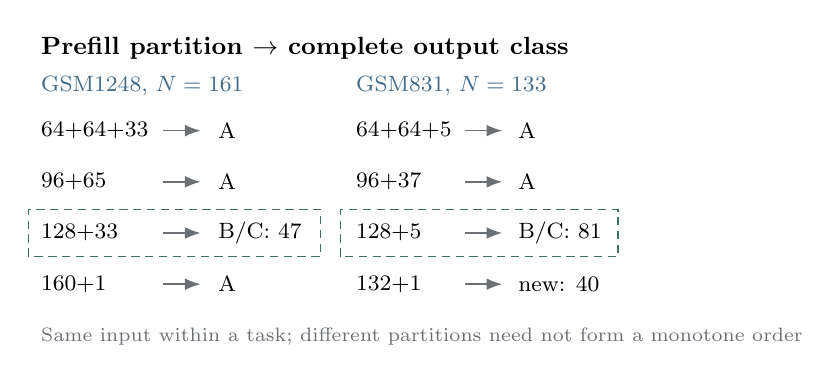
\begin{tikzpicture}[x=1cm,y=1cm,font=\footnotesize]
\node[anchor=west,font=\bfseries\small] at (0,3.35) {Prefill partition $\to$ complete output class};
\node[anchor=west,text=target] at (0,2.86) {GSM1248, $N=161$};
\node[anchor=west,text=target] at (4.0,2.86) {GSM831, $N=133$};
\foreach \y/\lab/\out in {2.3/{64+64+33}/A,1.65/{96+65}/A,1.0/{128+33}/{B/C: 47},.35/{160+1}/A}{
 \node[anchor=west] at (0,\y) {\lab};\draw[flow] (1.67,\y)--(2.15,\y);\node[anchor=west] at (2.25,\y) {\out};}
\foreach \y/\lab/\out in {2.3/{64+64+5}/A,1.65/{96+37}/A,1.0/{128+5}/{B/C: 81},.35/{132+1}/{new: 40}}{
 \node[anchor=west] at (4.0,\y) {\lab};\draw[flow] (5.51,\y)--(5.98,\y);\node[anchor=west] at (6.06,\y) {\out};}
\draw[qualified,densely dashed] (-.04,.70) rectangle (3.67,1.30);
\draw[qualified,densely dashed] (3.93,.70) rectangle (7.45,1.30);
\node[anchor=west,text=aux,font=\scriptsize] at (0,-.32) {Same input within a task; different partitions need not form a monotone order};
\end{tikzpicture}
}
\caption{Selected partition classes from the complete schedule table. A is whole prefill; B/C is the 128-split class. Numbers are first output differences from A. The map does not imply a universal 128-token threshold.}\label{fig:partition}
\end{figure}

\subsection{Projection and boundary reconstruction}
Native comparisons align actual embedding inputs, logical positions and the intended pre-attention RMS producer. Table~\ref{tab:projection} reports the layer-0 projection differences. Listing sibling projections in an audit sequence does not identify a unique first-cause kernel.
\begin{table}[t]\centering\small
\caption{Native layer-0 A/B projection differences. Values are maximum absolute differences for the stated tensors, not model-logit perturbation bounds.}
\label{tab:projection}
\begin{tabular}{@{}lrr@{}}\toprule
Projection&1248&831\\\midrule
Q&0&0.0207662582\\
K&0.0527343750&0.0703125000\\
V&0.0023193359&0.0021639541\\\bottomrule
\end{tabular}
\end{table}
Forty standalone calls compare RMS, scale/MUL and Q/K/V projections on two full/split operand geometries, with two repeats. Thirty-two pass native same-arm correspondence; eight scale/MUL calls fail because the captured input aliases a buffer already changed by an in-place consumer. Those failures remain excluded. RMS and the first task's Q controls agree bitwise, while admitted differing projection replays reproduce geometry sensitivity.

The common receiver restores sequence KV and positions, applies the native sampler to a complete 128,256-element initial FP32 vector, and reconstructs the empty generated prefix and pending token. Dynamic output buffers are rebuilt; opaque graph-cache pointers are not cloned. Sixteen own-path shams cover four inputs, both donor states and two repeats. Forty crosses then use three repeats per cell on the two affected tasks and two on the stable controls.
\begin{figure}[t]\centering\resizebox{\columnwidth}{!}{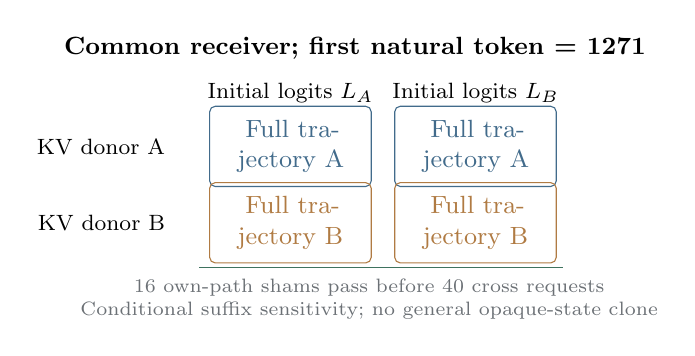
\begin{tikzpicture}[x=1cm,y=1cm,font=\footnotesize]
\node[anchor=west,font=\bfseries\small] at (0,3.35) {Common receiver; first natural token = 1271};
\node at (3.0,2.78) {Initial logits $L_A$};\node at (5.35,2.78) {Initial logits $L_B$};
\node[anchor=east] at (1.53,2.1) {KV donor A};\node[anchor=east] at (1.53,1.13) {KV donor B};
\foreach \x in {3.0,5.35}{
 \node[box,draw=target,text=target,text width=1.7cm,minimum height=.64cm] at (\x,2.1) {Full trajectory A};
 \node[box,draw=draft,text=draft,text width=1.7cm,minimum height=.64cm] at (\x,1.13) {Full trajectory B};}
\draw[qualified,line width=.6pt] (1.84,.56)--(6.46,.56);
\node[align=center,text=aux,font=\scriptsize] at (4.0,.16) {16 own-path shams pass before 40 cross requests\\Conditional suffix sensitivity; no general opaque-state clone};
\end{tikzpicture}
}
\caption{Admitted boundary0 cross for the affected tasks. All initial logits select 1271. The subsequent suffix follows the KV source under the same reconstructed receiver; stable controls retain their endpoint.}\label{fig:state}
\end{figure}

\subsection{Separate physical-work and cost boundary}
An earlier speculative actor executes a logical seed-plus-proposal verification as two occupied width-one target micrographs at $k=1$. The work-witness study retains 563 successful cycles and separate draft counts; one API-observer request failed a logging threshold and was not repeated. Its partial output is not a GPU timeline.

The original stock-relative cost campaign failed reference qualification. A later post-hoc full-output audit supports a different production-path pairing on 24 tasks and 240 repetitions: $R_{\rm prod}/C=0.719264$ and $M_{\rm match}/C=0.727927$, with every task regressing. Those negative same-output economics do not repair the original stock gate. They are not remeasured by the causal studies, and no completed component-time model is admitted.

\section{State components and decision frontiers}
\label{supp:composition}\label{supp:subsets}
\subsection{Selectors and complete endpoint matrix}
A denotes the historical whole-prefill state and B the partitioned state. Each intervention preserves recipient initial logits, natural pending-token consumption and the common receiver. Thirty-two EMPTY/ALL controls pass before the 160 subset requests. Table~\ref{tab:subsetmatrix} retains all 80 task/selector/direction coordinates; both process repeats agree. When donor and recipient natural endpoints coincide, a match is D rather than attributed to a distinguishable donor.
\begin{table*}[t]
\centering\small
\caption{All 80 distinct subset/direction coordinates. Both process repeats agree in every cell. Within each task the columns are A$\to$B and B$\to$A. B, C and D denote endpoint classes, not task-answer quality.}
\label{tab:subsetmatrix}
\begin{tabular}{@{}l*{8}{c}@{}}\toprule
 & \multicolumn{2}{c}{/1248} & \multicolumn{2}{c}{/831} & \multicolumn{2}{c}{/1011} & \multicolumn{2}{c}{/1249}\\
\cmidrule(lr){2-3}\cmidrule(lr){4-5}\cmidrule(lr){6-7}\cmidrule(l){8-9}
Selector & A$\to$B & B$\to$A & A$\to$B & B$\to$A & A$\to$B & B$\to$A & A$\to$B & B$\to$A\\\midrule
$K_0$       & B&D&C&C&C&C&D&D\\
$V_0$       & B&B&B&C&C&D&D&D\\
$K_0+V_0$   & B&D&B&C&C&D&D&D\\
All K       & D&B&C&C&C&C&D&D\\
All V       & D&B&C&C&C&C&D&D\\
Early KV    & D&D&B&C&C&D&D&D\\
Middle KV   & D&D&B&D&D&C&D&D\\
Late KV     & C&B&D&C&C&C&D&D\\
Prefix KV   & D&B&B&D&C&C&D&D\\
Tail KV     & D&B&B&D&C&C&D&D\\\bottomrule
\end{tabular}
\end{table*}
All 76 D requests change actual bytes. K-only or V-only layer0 selects $1/64$ of K/V value storage, excluding metadata. Early, middle and late groups contain 8, 16 and 8 layers. Prefix is $[0,128)$; tail is its complement, with five positions for /831. K is token-major and non-flash V feature-major, so each selector uses the actual storage strides. The source records separately retain selected bytes, changed bytes and numerical distances.

\subsection{Magnitude and common-prefix selection}
Table~\ref{tab:statenorm} reports differences computed from stored F16 values using the actual A-state norm. No increasing one-threshold rule perfectly separates these four endpoint labels: a smaller overall perturbation can accompany divergence while a larger one does not. This is a finite counterexample to a magnitude-only explanation, not an alternative predictor.
\begin{table}[t]\centering\small
\caption{Full-KV differences, B relative to A, computed from stored F16 values. Endpoint labels refer to natural A/B continuations on four exposed inputs.}
\label{tab:statenorm}
\begin{tabular}{@{}lrrl@{}}\toprule
Task & Relative $L_2$ & Max. absolute & A/B endpoint\\\midrule
/1248 &0.006488689&0.255859375&Different\\
/1249 &0.006748138&0.246093750&Same\\
/1011 &0.006887112&0.265625000&Same\\
/831  &0.010452955&1.332580566&Different\\\bottomrule
\end{tabular}
\end{table}
For each task, recipient and panel, the frontier $t^*$ is the first output at which the four natural trajectories cease to agree. Their consumed prefix is identical at that point. L0 and POSITION have separate frontiers; /831 recipient A reaches them at 40 and 81 respectively. Later vectors cannot fill an earlier missing comparison.

Archived captures support 44 of 112 planned repeat-level contrasts, with 22 agreeing pairs. The 68 incomplete comparisons contain 272 missing panel entries or 240 distinct arm/repeat/position vectors, because some arms are shared. A vector hash or top-two scores do not replace full logits. Output zero uses the frozen initial logits and needs no additional forward. Table~\ref{tab:frontier} retains every available frontier contrast.
\begin{table*}[t]\centering\small
\caption{All available frontier contrasts. L0 components are K/V; POSITION components are prefix/tail. Both historical repeats agree. Values are rounded to six decimals. Token pairs are fixed within each panel; direction-dependent coordinates must be canonicalized before comparing signs.}
\label{tab:frontier}
\begin{tabular}{@{}lllr rrrr@{}}\toprule
Task&Direction&Panel&$t^*$&$\Delta_1$&$\Delta_2$&$I$&EMPTY margin\\\midrule
1248&B$\to$A&L0&47& .059744& .088148&-.135864&.066515\\
1248&A$\to$B&L0&47& .025909& .033445&-.019032&.010706\\
1248&B$\to$A&POSITION&47& .078003& .095778&-.096560&.066515\\
1248&A$\to$B&POSITION&47&-.018557&-.000782& .096560&.010706\\
831&B$\to$A&POSITION&81&-.095177&-.062551& .238718&.013084\\
831&A$\to$B&L0&81& .118263& .172575&-.049446&.067905\\
831&A$\to$B&POSITION&81& .143541& .176167&-.238718&.067905\\\bottomrule
\end{tabular}
\end{table*}
For /1248 B$\to$A L0 at 47, the additive joint prediction is $0.08137702941894531$, the actual joint is $-0.05448722839355469$ and $I_{KV}=-0.1358642578125$. Full-vocabulary argmax is 220/220/832/220. At output46, the same fixed-pair residual is $-0.13482666015625$, but the actual top two are 11/220 with margin $8.017614364624023$; the frontier pair 220/832 is not that position's top two. Cross-position comparison is descriptive.

At output1 of /1011, EMPTY margins are $0.561777115/0.549312592$, maximum observed $\epsilon_\infty=0.207827211$, and every arm satisfies $m>2\epsilon_\infty$ and selects 11886. The mixed trajectories later diverge at 10, whose adjacent full vectors are missing. For /1249 the corresponding margins are $0.959617615/0.936807632$, maximum $\epsilon_\infty=0.194167793$, and every observed arm selects 1505. This sufficient top-1 condition applies only at the measured position.

\subsection{Direction symmetry and independent conditions}
For complete states $(A_P,A_T)$ and $(B_P,B_T)$, reversing donor and recipient permutes the POSITION quartet from AA, BA, AB, BB to BB, AB, BA, AA. When the actual state, prefix and receiver agree under this mapping,
\begin{equation}
\boldsymbol I=\boldsymbol z_{\rm ALL}-\boldsymbol z_P-\boldsymbol z_T+\boldsymbol z_{\rm EMPTY}
\end{equation}
is invariant. The scalar $I(u)-I(r)$ changes sign when $(r,u)$ is reversed. The audit checks actual state, FP32 vectors, prefixes, sampling conditions and F64 bytes in all 12 available direction pairs. For /1248 at47 both directions give $-0.09655952453613281$ in pair order $(220,832)$, despite opposite original signs.

Of the 44 oriented repeat rows, 24 are POSITION and 20 L0. Accounting for direction symmetry and two repeats gives six POSITION and ten oriented L0 conditions, still only four underlying inputs. L0 has different surrounding recipient states and is not collapsed by the POSITION identity.

\subsection{Acquisition failure and data scope}
A new acquisition attempted one request with a registry key missing recipient identity. The planned EMPTY B$\to$A imported B rather than A, completing 127 decodes before failing the input check. It is neither a qualified EMPTY nor an ALL sample; 167 slots were unstarted. The later CPU revision repairs request assembly without new native data. The 54 unique FP32 vectors and 16 residual vectors support the historical 44 contrasts; no missing frontier or independent-machine GPU replication is supplied by that revision.

\section{Natural-execution port and backend audit}
\label{supp:pilot}
\subsection{Design and complete exploratory endpoints}
The natural pilot keeps the original ordinary UB128/capacity-one reference R. R\_SHADOW tests the rebuilt actor without replacing R. Candidate prefill uses reference128 or bulk512 organization, MQ attention and capacity4. Six speculative arms use continuation MQ/PQ/QB, target UB4, $k=1$ and the same draft; two arms are draft-free. Every request starts from its prompt without imported state.

The planned 80 requests are eight original R, four shadow counts, four shadow diagnostics, 32 candidate counts and 32 candidate diagnostics. It stops with 49 attempts, 48 complete, one interrupted and 31 unstarted. Table~\ref{tab:pilot} preserves all 14 endpoint counterexamples. The reference and shadow outputs agree, but candidate observer pairs are incomplete. The q1 branch bypasses the multi-query transformation, so draft-free QB-labelled agreement does not qualify lifted QB.
\begin{table}[t]\centering\small
\caption{Complete candidate counts endpoints observed before stopping. Values are first differing output indices from original R; ``='' denotes an equal complete cap128 endpoint. Candidate observer pairs are incomplete. The execution-contract limitation prevents qualification of this panel.}
\label{tab:pilot}
\begin{tabular}{@{}lrrrrr@{}}\toprule
Arm&/1248&/831&/1011&/1249&Matches\\\midrule
$M_{B,\QB}$&47&81&=&=&2/4\\
$M_{R,\QB}$&=&=&=&=&4/4\\
$C_{B,\MQ}$&47&40&10&=&1/4\\
$C_{B,\PQ}$&47&81&=&=&2/4\\
$C_{B,\QB}$&47&40&10&=&1/4\\
$C_{R,\MQ}$&=&40&10&=&2/4\\
$C_{R,\PQ}$&=&=&=&=&4/4\\
$C_{R,\QB}$&=&81&10&=&2/4\\\bottomrule
\end{tabular}
\end{table}
The frozen monitoring declaration requires 100ms request-period VRAM sampling. The original R instead supplies four checkpoints, with maximum gaps 2874--3033ms. The mismatch is detected while the 49th request is active; only its owned worker is terminated. No sampled threshold violation was observed, but the original declaration remains unmet. P2/P3 are not executed and qualified speedup remains null. The 8,110 caller events, full times and raw accounting are retained in the ancillary record.

The available candidate diagnostics contain histograms but no ordered, phase-bound multirow VERIFY witness, leaving actual multirow placement unresolved. Descriptive request times include the new actor's observation, lifecycle and phase-management costs as well as attention.

\subsection{Independent representation audit}
The follow-up uses the same frozen CPU numerical libraries across 144 development and 288 locked held-out synthetic fixtures. It covers $q\in\{1,2\}$, key extents 127/128/129/255/256/257, head pairs $(8,8),(8,1),(32,8)$, $d=128$, and compact or legally offset model-permuted Q. Three nonempty masks and two fixed data patterns give 72 geometries and 432 fixtures; MQ/PQ/QB require 1,296 CPU graph evaluations. Held-out here refers to synthetic test conditions, not new model prompts.

An independent integer oracle checks addresses, contiguous-group GQA, mask columns and output recovery. Four injected faults are detected. A separate FP64 scalar oracle uses stored inputs. Structured one-hot and single-valid-key tests have exact expectations. No strict assertion, crash or nonfinite failure occurs. General differences remain descriptive: maximum absolute error is zero at QK on the dyadic inputs, $5.3608031\!\times\!10^{-9}$ at softmax, and $5.5132505\!\times\!10^{-5}$ at AV/final output. No post-hoc tolerance defines a general numerical pass. F16-representable dyadic data do not establish generic F32 reduction invariance.

The complete historical endpoints satisfy $M_{B,\QB}=C_{B,\PQ}$, $M_{R,\QB}=C_{R,\PQ}$ and $C_{B,\MQ}=C_{B,\QB}$ on all four windows. On /1011, $C_{R,\MQ}$ and $C_{R,\QB}$ both first differ at10 but have different full endpoints. These relations do not establish common operands, KV or acceptance traces.

\subsection{Version-bound support semantics}
Seven core backend/header hashes match the archived build manifest and the numerical DLLs are unchanged. The frozen \texttt{ggml\_backend\_vk\_device\_supports\_op} rejects the reviewed QK and AV shapes because their fourth source extents are $(1,2)$. The complete source identity and line location are in \texttt{anc/portability111.json}. Unbound shader bodies are excluded from arithmetic attribution.

The descriptor checker rejects the unequal fourth extents and leaves other cases unresolved because equality is only one necessary admission condition. This CPU/source analysis identifies the backend change required before a same-backend numerical comparison. Actual routing and fallback remain unknown, and the stopped pilot retains its failed qualification.

\section{Mapping, representation and observer controls}
\label{supp:followupmapping}
The post-replication mapping studies retain distinct references, input sets, runtimes and timers~\cite{mappingrecords,b570compactrecords}. Their results are not additional samples of the original E2 experiment. The full scientific heads and paths are in \texttt{anc/source\_manifest.json} and the follow-up evidence index.

\subsection{Input lifetime and software controls}
The original RTX allocation allowed later AV and ordinary-output nodes to overwrite storage holding K/V. Address and byte witnesses, re-upload interventions and return to the original allocation localized this failure. Independent persistent input storage restored repeated input and output bytes. This repair establishes valid repeated execution; it supplies no accelerator result.

Balanced PQ/QB/QH comparisons use identical QB\_A/QB\_B controls. The core $q=2,4$ panel yields QB\_A/QH=0.900826, with 19 of 24 geometries supporting lower QB cost under the declared descriptive screen and five unresolved. A/A pilot envelope reduction to a median 2.762\% does not establish 2\% precision for each geometry. A selector predicts all 12 held-out synthetic mean directions but costs 1.010298 times fixed QB once the measured lookup is charged; its estimate is an offline phase sum, not an integrated request.

CUDA Graph ON is established through capture, instantiation and replay in instrumented hosts. Clean hosts share the graph/runtime identity without loading the observer. The ON/OFF intervention reduces QB\_A completed-graph cost to 0.615--0.849 of OFF. Profiling traces identify path changes, but kernel durations do not supply a union of busy time or a request critical path.

\subsection{Fixed-logical-input padding and cost windows}
Logical-length-preserving padding keeps original mask columns and appends finite zero K/V with fully masked keys. L1023/S1024 fails all four reference qualifications despite reaching three kernels at the first observed execution. L1023/S1025 qualifies all four, retains eight kernels and costs 1.014783/1.014974 times the two native controls. L1024/S1025 and L1024/S1026 also fail the exact reference. All failed paths stop at the first mismatch; no clean steady-state benefit is reported for them. Source-to-DLL correspondence for the internal RTX divergence remains unknown.

The complete RTX Q transaction begins with common permuted host Q and includes copy/transpose, Q upload/completion, graph replay/synchronization and full ordinary readback. For $q=2,4$, compact-QH/QB\_A is 1.002216/1.001598 and compact-QH/QB\_B is 1.008295/1.004167. K/V/mask are resident and targets preallocated; the interval excludes natural Q generation and continuing KV updates.

The B570 equal-head panel instead uses Hq/Hkv=8/8, $d=128$, key1023/1024/1025 and $q=1,2,4$. Its narrow admission repair enables the existing batch-broadcast shader without K/V REPEAT. Three fixed input sets and three process sessions, balanced over both identical QB controls and QH, give a resident-graph difference of $-1.028\,\mu$s [$-2.177,+0.067$]. The separately measured complete representation transaction gives $-1.518\,\mu$s [$-4.168,+0.916$], ratio 0.992244 [0.979908,1.004691]. These are descriptive adjusted intervals from three process clusters on one device/date; all practical-effect screens remain unresolved. The 43,740 transactions are technical repetitions, not independent workloads. The two windows cannot be subtracted to isolate transfer cost.

\subsection{Request relevance and observer integrity}
The first B570 Qwen3 request bridge is a separate q1/key256/GQA32:8 observation. It does not exercise the equal-head near1024 micrograph. Serial per-operation logging adds about 12\% median decode overhead and fails its 10\% observer screen. Concurrent logging initially omits the terminal interval and includes inactive-node labels; terminal timestamps and the executor's active-node predicate repair those faults.

The final same-DLL clean/profile/clean medians are 27.6675/29.6058/27.6794 ms, so the observer still adds about 7\%. Each final context table counts 16 output projections and 5,004 QK, softmax, AV and CONT operations each. The third-context GPU subtotal is 3.490070 s over prefill and continuation. Pure QK/softmax/AV contributes 2.8005\%, or at most 2.8026\% when the mixed group is included; the core excludes projections, RoPE and KV updates. Quantized matvec/fused groups contribute 92.5152\% and contain both attention projections and FFN. These diagnostic fractions are not clean request shares or a bandwidth diagnosis.

\section{Historical finite-panel service results and prefill closeout}
\label{supp:service}
\subsection{Panel identities and qualification}
Table~\ref{tab:servicecontracts} lists the two service contracts. Each panel has four exposed inputs, $k=1$, 32/8 target GQA, F16 KV and actual two-query verification in all 36 target layers. The draft and target models are Qwen3-0.6B and Qwen3-8B Q8\_0. Model/tokenizer hashes and exact driver identities are pinned separately; the shared family names do not make these a paired GPU experiment.

\begin{table*}[t]\centering\small
\caption{Distinct service contracts. The entries describe the recorded experiments, not recommended production configurations.}
\label{tab:servicecontracts}
\begin{tabularx}{\textwidth}{@{}p{3.0cm}YY@{}}\toprule
Property & RTX service study & B570 formal request study\\\midrule
Reference and inputs & New R/PQ full-logit references, historical native endpoints; MBPP/413, GSM8K/120,322,443 & Prospective q1 reference; HumanEval/38,65,115,127 with their recorded chat formatting\\
Output window & Native EOG or cap128 & Native EOG or cap64\\
Target/draft capacity & R target UB1; speculative target UB4; draft UB1 & Target verification UB4; draft UB1; serialized q1 prefill\\
Context and host policy & Context1024, 24 host threads & Context1024, eight context thread parameters\\
Measurement & 64 requests in four timing processes; 64 explicit warmups & 64 requests in four timing processes; 16 explicit warmups\\
Qualification & Eight reference requests and 12 independent qualification requests; 1,106+1,794 vectors & 12 qualification requests; 346 saved PQ/QB full-logit pairs\\
Primary window & Fresh-context creation/reservation through prefill, generation, state/synchronization and teardown & Same declared service components; separate private driver and prefill policy\\
Excluded / separately charged & Shared model loading, post-timer comparison and raw-file I/O & Shared model loading, post-timer comparison and raw-file I/O\\\bottomrule
\end{tabularx}\end{table*}

The RTX source/driver registration precedes every model start; its independently generated R/PQ reference is sealed before qualification, and the qualification record is sealed before timing~\cite{rtxservicerecords}. R uses its matching reference; PQ and QB use the matching PQ target/draft vectors, including rejected verification rows. Their complete speculative traces also agree. This does not assert that every internal PQ value equals a serial R value. Query geometry and mask extents/strides are observed, whereas visible-key counts are derived from the registered causal positions. No operator readback is inserted into the natural CUDA graph.

The B570 AV repair first passes six synthetic key256/512 by $q=1,2,4$ coordinates with unchanged PQ stage files, then a model integration passes one exposed 16-token bridge. Its first cost pilot preserves a 5.123483-second discrepancy between identical PQ arms. The apparently favorable aggregate is not promoted into a speedup. A separately registered four-input panel uses a 64-token cap and natural EOG, and qualifies complete R/PQ/QB endpoints, 346 PQ/QB vectors and full speculative cycle traces before timing~\cite{b570gqarecords,b570servicerecords}. The old Llama Q6\_K references and their failures remain separate.

\subsection{Every input and paired block}
\begin{table*}[t]\centering\small
\caption{All input-aggregate service ratios. Four sessions contribute to each row. A/A is the ratio of two identical PQ controls. Lower QB ratios favor QB. Inputs are different between platforms.}\label{tab:serviceinputs}
\begin{tabular}{@{}llrrrr@{}}\toprule
Platform & Input & Output / stop & QB / dual-PQ & QB / R & PQ\_A / PQ\_B\\\midrule
RTX & MBPP/413 & 34/EOG & 0.988025 & 0.608126 & 0.947919\\
RTX & GSM8K/120 & 128/CAP & 1.004279 & 0.578678 & 0.956661\\
RTX & GSM8K/322 & 128/CAP & 0.963695 & 0.610027 & 0.990391\\
RTX & GSM8K/443 & 128/CAP & 1.001663 & 0.535651 & 0.964986\\
\textbf{RTX} & \textbf{Equal-weight mean} & --- & 0.989284 & 0.582325 & ---\\\midrule
B570 & HumanEval/38 & 64/CAP & 0.994638 & 2.597826 & 0.999532\\
B570 & HumanEval/65 & 53/EOG & 0.992003 & 2.652017 & 0.997703\\
B570 & HumanEval/115 & 41/EOG & 0.997281 & 2.619785 & 0.999881\\
B570 & HumanEval/127 & 64/CAP & 0.996663 & 2.609733 & 0.992463\\
\textbf{B570} & \textbf{Equal-weight mean} & --- & 0.995144 & 2.619763 & ---\\\bottomrule
\end{tabular}
\end{table*}

\begin{table*}[t]\centering\footnotesize
\caption{Every input/session block from the two service panels. Each platform has its own input set; adjacent rows do not form cross-platform pairs. Exact source blocks are included in the ancillary CSV files.}\label{tab:serviceblocks}
\begin{minipage}[t]{.485\textwidth}\centering
\textbf{RTX}\par\vspace{4pt}
\setlength{\tabcolsep}{3pt}\begin{tabular}{@{}rlrrr@{}}\toprule
$s$ & Input & QB/PQ & QB/R & A/A\\\midrule
0 & M/413 & 1.139826 & 0.860710 & 0.995684\\
0 & G/120 & 0.945850 & 0.626761 & 0.948687\\
0 & G/322 & 0.923908 & 0.620302 & 1.002893\\
0 & G/443 & 0.922590 & 0.536318 & 0.937857\\
1 & M/413 & 1.037841 & 0.605209 & 1.018199\\
1 & G/120 & 1.060687 & 0.598746 & 0.928511\\
1 & G/322 & 0.964679 & 0.643793 & 1.133151\\
1 & G/443 & 1.095851 & 0.587714 & 0.908679\\
2 & M/413 & 0.867052 & 0.507936 & 0.836860\\
2 & G/120 & 1.075364 & 0.574851 & 0.996817\\
2 & G/322 & 1.063244 & 0.656443 & 0.950265\\
2 & G/443 & 1.031135 & 0.530409 & 1.012026\\
3 & M/413 & 0.929090 & 0.516898 & 0.951652\\
3 & G/120 & 0.942870 & 0.519815 & 0.953907\\
3 & G/322 & 0.910152 & 0.528264 & 0.890920\\
3 & G/443 & 0.965632 & 0.492411 & 1.005416\\
\bottomrule\end{tabular}\end{minipage}
\hfill
\begin{minipage}[t]{.485\textwidth}\centering
\textbf{B570}\par\vspace{4pt}
\setlength{\tabcolsep}{3pt}\begin{tabular}{@{}rlrrr@{}}\toprule
$s$ & Input & QB/PQ & QB/R & A/A\\\midrule
0 & HE/38 & 0.994435 & 2.594996 & 1.000263\\
0 & HE/65 & 0.994347 & 2.670002 & 0.998378\\
0 & HE/115 & 0.997636 & 2.622364 & 0.999695\\
0 & HE/127 & 0.998560 & 2.603504 & 1.001035\\
1 & HE/38 & 0.995388 & 2.601387 & 0.997047\\
1 & HE/65 & 0.990654 & 2.645055 & 1.001826\\
1 & HE/115 & 0.997896 & 2.619781 & 1.000689\\
1 & HE/127 & 0.997328 & 2.604889 & 0.998169\\
2 & HE/38 & 0.997377 & 2.602636 & 1.001209\\
2 & HE/65 & 0.992339 & 2.647094 & 0.997665\\
2 & HE/115 & 0.996576 & 2.619385 & 0.998640\\
2 & HE/127 & 0.998198 & 2.602524 & 0.998604\\
3 & HE/38 & 0.991360 & 2.592299 & 0.999614\\
3 & HE/65 & 0.990676 & 2.645998 & 0.992961\\
3 & HE/115 & 0.997017 & 2.617613 & 1.000503\\
3 & HE/127 & 0.992578 & 2.628099 & 0.972324\\
\bottomrule\end{tabular}\end{minipage}
\end{table*}

The tables and Figure~\ref{fig:servicepanels} are generated from the saved block records. RTX blocks retain all four arm service times, permitting direct recomputation of each ratio. B570's table retains the archived paired ratios; recomputing their geometric means is not reconstruction from unprovided raw service logs. \texttt{anc/check\_closure.py} verifies exact Git blob identities, weights, input/session coverage, ratios, plot coordinates and printed cells. Neither table supplies full raw logits.

The primary layout estimator gives equal weight to each input and session in log space. Its A/A criterion is the largest absolute per-input geometric-mean PQ\_A/PQ\_B deviation from one, not the largest individual block deviation. The finite engineering screen also requires more than 2\% reduction and all session aggregates below one. RTX session ratios are 0.979094, 1.038635, 1.005512 and 0.936718, and the A/A criterion is 5.208\%. B570 session ratios are 0.996243, 0.995313, 0.996120 and 0.992904, with A/A criterion 0.754\%; its 0.486\% layout point reduction is below 2\%. Neither panel passes the practical layout screen.

All 16 RTX QB/R blocks are below one and all 16 B570 QB/R blocks exceed one. Aggregate ratios are 0.582325 and 2.619763 respectively. RTX dual-PQ/R is 0.588633, showing that the speculative-policy benefit is already present with PQ. The 41.8\% RTX reduction describes lower service time, not a 41.8\% increase in token throughput. The inverse ratio is a different quantity. No confidence interval is manufactured from four exposed inputs and process repeats.

Warmups are separately recorded, but their presence alone establishes neither cold-driver behavior nor warmed state for all shapes. B570 uses the old 16-token key256 request for warmup; key512 pipeline persistence across processes is uncontrolled. The RTX panel warms each input/arm. Continuous exclusive device ownership is not established in either study. All blocks and reversals are retained; no outlier deletion or significance-driven extension is used.

\subsection{Draft-policy counterfactual and completed prefill follow-up}
The B570 thread-parameter study fixes the PR134 QB references and changes draft context parameters from 8 to 1 while keeping the target at 8. All 346 vectors and endpoints/state traces remain unchanged. Four timing processes yield 64 measurements plus 16 warmups. DRAFT1/dual-baseline service is 1.003994, DRAFT1/R is 2.633056 and the A/A criterion is 0.793\%. The session ratios 0.998803, 1.007142, 1.010567 and 0.999512 do not support a practical improvement~\cite{b570policyrecords}. A temporary ggml pool object in an OpenMP build does not establish per-call creation of OS threads; the one-task GET\_ROWS/SET\_ROWS plan can clamp effective workers before the parameter takes effect.

The same reviewed commit also contains a draft-prefill submission follow-up. Its first attempt fails an observer-axis check; this failure is retained. A prospective observer-only repair checks the consumed QK tensor and all four inputs then qualify, with 346 matching logits, one draft-prefill API call and physical prefill $q=1$. A later registered closeout completes this cost comparison under its separate CPU-draft service contract~\cite{b570prefillrecords}. It records 156 requests: four calibration, 24 qualification, 64 matched warmups and 64 measurements. SUBMIT/dual-baseline is 0.999161, a 0.084\% point reduction against 0.369\% input-aggregate A/A and a 2\% practical floor. One session favors the baseline. Fewer submissions therefore do not establish lower complete service cost, and QB/thread8 remains the baseline. SUBMIT/R is 1.203678 in this later contract; it cannot be compared with PR134's 2.619763 as a controlled improvement because device placement and service policy differ. The recorded helper-process reservation was not a complete observed count; full resource-protocol compliance is not established. The valid negative cost result and that accounting limitation are both retained.

\subsection{Evidence and execution accounting}
The RTX study completes 12 native processes and 148 requests: eight references, 12 qualification, 64 measured and 64 warmups. All native exits and cleanup are recorded, with no scientific retry. The conditional 24 profiling slots remain unstarted under the registered stopping rule. Native parent lifetime is 446.746733 seconds; GPU-active time is unmeasured. The preparation staging failure is retained, and its earlier compiler lifetime was not captured.

The locally retained RTX archive contains 3,110 members and 2,900 vectors and is 2,270,281,687 bytes. The originating host reports reopening and hashing every member. The present manuscript package contains reported blocks, derived values, source identities and the original consistency inputs; it does not contain that full native archive. Local restoration, GitHub compact-record reconstruction and independent full-raw access are different evidence levels. B570's original full vectors also remain separately held.

\section{Matched deployment, input transfer and native reproduction}
\label{supp:followup}
\subsection{Frozen matched design and uncertainty}
The RTX bridge freezes at \texttt{30ad53be} before six formal process sessions. Its twelve-input panel is MBPP/123,140,255,401,413,418 and GSM8K/111,120,1308,141,322,443. Each session measures every input in four cells and three arms, giving $6\times12\times4\times3=864$ measurements; twelve warmup requests per session add 72. All 936 requests complete without formal retries, missing slots or outlier removal. Each cell occupies each order position three times per session. Each cell/session uses every three-arm permutation twice; each input/cell uses all six permutations across sessions.

The primary estimator is the exponential of the equal-input, equal-session mean of $\log[T_{\QB}/\operatorname{mean}(T_{\PQ_A},T_{\PQ_B})]$. The registered 20,000-resample bootstrap jointly resamples the six session vectors, preserving the four paired cells. Each cell uses a 98.75\% percentile interval, yielding nominal 95\% family coverage across four primary cells. Practical success additionally requires an upper ratio below 0.98, a point reduction above both 2\% and the input-aggregate A/A imbalance, and improvement in every session. With six sessions on one date, these intervals describe process-session variation on that host; date-level uncertainty is unmeasured.

The absolute arithmetic PQ/QB service means are 1.646575/1.631283 seconds for $k=1$ resident, 1.358022/1.272156 for $k=3$ resident, 1.690768/1.655382 for $k=1$ fresh and 1.371483/1.307389 for $k=3$ fresh. Ratios of these arithmetic means need not equal the primary geometric paired estimate. All per-input regressions, session signs, omit-one-session, chronological and pointwise $t$ sensitivities remain in the archived analysis. The secondary $k3/k1$ ratios of layout ratios are 0.950119 resident and 0.972137 fresh; lifecycle contrasts are 0.986740 at $k=1$ and 1.009607 at $k=3$, with pointwise intervals spanning one for both lifecycle contrasts. The interaction is exploratory.

\subsection{Preserved engineering attempts and observation cost}
A 25-request pilot precedes qualification. The first qualification attempt completes 135 requests before a Windows aggregate-file replacement failure leaves 69 slots unexecuted. A recording-only correction creates a new executable identity, and all 204 qualification requests are rerun before freezing formal timing. No formal samples are pooled across builds. A counter pilot has an unresolved approximately 2.9\% difference, so the additional counters and heavy callback/logit capture are off during formal timing. Common driver bookkeeping, phase timers and inherited backend logging remain included. Actual CUDA capture/replay/fallback activity is not fully recorded.

\subsection{Previously unexposed panel and stopped families}
The input-transfer study is separately frozen and does not share the bridge's exposed-input claim. It reaches 33 of 36 family/input cells, representing 20 of 21 distinct tasks. Independent compact reconstruction reconciles 1,018 completed and 758 unexecuted request slots; the two qualified families contribute 384 measurements and 384 warmups. No successful Llama subset is timed after its reference counterexample. Initial missing raw-offset metadata is retained; a heavy-observer correction and causal rules are fixed before held-out selection. The native-fast path fails old calibration for SmolLM2/Llama and held-out GSM8K/70 for Qwen3. Source-pinned counterexample token IDs, dispositions and all cost rows accompany the paper.

\subsection{Native evidence and access}
RTX restores 3,542 original and 3,537 metadata4 source members, rebuilds core/frontend objects, and retains the pinned numerical DLLs. A real Qwen3 layer0/q3 fixture passes original/rebuilt MQ/PQ/QB replay with two repeats; six original/rebuilt HTTP R/PQ/QB requests match the historical endpoint. Compact native fixture and formal-record archives are in the result branch; the full 38,078-file raw directory remains separately held.

B570 rebuilds all five numerical libraries and 147 shader translation units from source. A new HumanEval/115 layer0/q2/key512 capture and its first-query q1 slice pass 16 stage comparisons. The ordinary four-input R/PQ/QB panel matches 914 historical complete vectors plus outputs, stops and state; copied-directory execution passes again. A diagnostic capture/supervision correction retains identical numerical DLL hashes. All 21 model requests and two stage workers are accounted for; nine additional cumulative Job processes lack identities/lifetimes. These resource limits do not change the recorded numerical comparisons. The full 1.37 GB compressed archive remains on the source host; Git includes the real stage fixture and receipts. This reproduces PR134's two-model Vulkan contract, not PR143's later CPU-draft service policy.

\texttt{anc/followup\_20261026/} carries exact compact records, source pins, derived tables and a read-only reconstruction path. The present manuscript revision performs CPU analysis only. Native build and replay results above are the platform executions recorded in the cited campaigns.

\balance
\section{Reproduction and evidence access}
\label{supp:reproduction}
The source package builds the article and supplement from \texttt{main.tex}. It includes editable figures, all reported cost/state matrices, original RTX session tables, later service blocks and recovered E2 request times. Standard-library scripts reconstruct the primary bootstrap, absolute request costs, repair--draft contrasts and secondary session sensitivity. Source hashes bind copied inputs to their campaign records. Derived JSON permits one adjacent binary64 value to accommodate platform math-library rounding; source bytes, integer counts and generated TeX remain exact.

\texttt{anc/runtime\_reproduction/} supplies CPU interface tests and archived implementation sources/patches with provenance. These expose the query/mask mapping, phase/cache contract and scoped AV repair for inspection. Native reruns additionally require the matched runtime source/build routes, numerical libraries, models and capture fixtures listed in that directory. The CPU package is executable on its own; it does not execute the GPU experiments.

\texttt{anc/source\_manifest.json} pins each campaign. Original RTX evidence is sealed at \texttt{f997262d}, the B570 support audit at \texttt{9fafc4ba}, RTX service at \texttt{9868acfb}, and B570 service/policy at \texttt{51febadd}/\texttt{e44c4df0}. Complete runtime and tensor archives are separately held; the manuscript package makes reported-data reconstruction independent of them. \texttt{anc/historical\_disposition.csv} and \texttt{anc/editorial\_archive/} retain the 28 legacy groups and later failures. The archived \texttt{dae5aea9} AV model remains a same-policy parity control, with no hardware-performance claim.

This revision reanalyzes existing measurements and adds no native execution. Generated TeX resides in \texttt{tables/}, outside \texttt{anc/}, so article compilation does not depend on ancillary-data handling. The README gives the full check/build commands and separates CPU validation from the dependencies needed for a native rerun.

\end{document}
